\chapter{Training Private Models That Know What They Don't Know}
\label{ch:sptd_dp}

% \paperref{\bibentry{rabanser2023training}}

\begin{paperref}
\normalfont
The contents of this chapter consist of research and results taken from: \emph{\bibentry{rabanser2023training}}
\end{paperref}


\section*{Summary}

Training reliable deep learning models which avoid making overconfident but incorrect predictions is a longstanding challenge. This challenge is further exacerbated when learning has to be differentially private: protection provided to sensitive data comes at the price of injecting additional randomness into the learning process. In this work, we conduct a thorough empirical investigation of selective classifiers---that can abstain under uncertainty---under a differential privacy constraint. We find that some popular selective prediction approaches are ineffective in a differentially private setting because they increase the risk of privacy leakage. At the same time, we identify that a recent approach that only uses checkpoints produced by an off-the-shelf private learning algorithm stands out as particularly suitable under DP. Further, we show that differential privacy does not just harm utility but also degrades selective classification performance. To analyze this effect across privacy levels, we propose a novel evaluation mechanism which isolates selective prediction performance across model utility levels at full coverage. Our experimental results show that recovering the performance level attainable by non-private models is possible but comes at a considerable coverage cost as the privacy budget decreases.

\section{Introduction}
\label{sec:intro}

% \djcomment{Taking a stab at an alteranative more concise intro here: State of the art machine learning models are gaining rapid adoption. However, major challenges remain to be addressed, in particular around the reliability of these models and their ability to protect privacy of the individuals whose data they were trained on, particularly in safety critical domains like healthcare. In particular, approaches that offer strong theoretical guarantees around privacy, i.e., differential privacy, lead to substantial drops in accuracy of trained models. These drops in accuracy can particularly impact underrepresented subgroups in that data (provide refs), since differential privacy makes models insensitive to small changes in tail populations. Furthermore, differential privacy necessarily increases the randomness in model ouptuts due to the inherent randomness in mechanisms that achieve differential privacy. However, there }

% \djcomment{
% In this paper, we propose an approach to address both the reliability and privacy problems in deep learning models via differentially private selective classification. We examine various approaches for selective classification and their performance under differential privacy, and demonstrate that a recently proposed approach based on examining the behavior of predictions for a test example over checkpoints generating during the differentially private learning algorithm. This approach has clear advantages in the private settings as it does not requre training any additional parameters for a rejection model or an ensemble of models, both of which have a detrimental impact on privacy. 
% }

% \djcomment{
% Since differential privacy has a substantial impact on accuracy of learning algorithms, we propose a novel metric to quantify the gains that can be attributed to the selective classification component of the system, and separate this from gains that come from improvements to accuracy of the classifier overall (without selective prediction). This allows us to both quantify the difficulty of achieving gains in differentially private selective classification, and demonstrate the benefits of our checkpoint-based approach.  
% }

% \djcomment{
% Our experimental results clearly demonstrate the value of differentially private selective classification can lead to significant improvements in the tradeoff between accuracy and coverage (the fraction of examples the selective classifier). 
% }

%\stephan{Will rewrite this following paragraph}

% Current state-of-the-art machine learning (ML) models have attained remarkable performance on a multitude of prediction tasks, ranging from ... over ... to ....\todo{You can remove the previous sentence - too vague} 
% Contemporary machine learning ML models offer strong generalization performance to unseen inputs, it has also been shown that this level of performance can be partly attributed to the memorization capability of contemporary over-parameterized models.%\my{Given my expectation that this is about selective classification, the jump start to "memorization" was a logical leap for me.} 
% However, while memorization seems to boost performance, it can simultaneously impair the privacy of the training data. To showcase this shortcoming, past works have (i) demonstrated membership inference attacks to determine the presence of particular data points in the training set; and (ii) enabled extraction of private data used for model training. In order to prevent such attack vectors, $(\epsilon, \delta)$ differential privacy (DP) has emerged as the current de-facto standard used to limit the amount of privacy leakage from individual data points. 
%Training models with differential privacy ensures that the information content that can be acquired from individual data points is bounded while patterns present across multiple data points can still be extracted.\my{this paragraph is about of the value of DP-learning. I think this is valid, but maybe too long for a neurips intro.}
State of the art machine learning (ML) models are gaining rapid adoption in high-stakes application scenarios such as healthcare~\citep{challen2019artificial, mozannar2020consistent}, finance~\citep{vijh2020stock}, self-driving~\citep{ghodsi2021generating}, and law~\citep{vieira2021understanding}. However, major challenges remain to be addressed to ensure trustworthy usage of these models. One major concern in sensitive applications is to protect the privacy of the individuals whose data an ML model was trained on. %Failure of ensuring privacy protection can lead to (i) membership inference attacks to determine the presence of particular data points in the training set; and (ii) extraction of private data used for model training. 
To prevent privacy attacks on ML models, $(\varepsilon, \delta)$ differential privacy (DP)~\citep{dwork2014algorithmic} has emerged as the de-facto standard with widespread usage in both academic and industrial applications. %to limit the amount of privacy leakage from individual data points. 


While the introduction of DP successfully protects against privacy attacks, it also limits model utility in practice. For instance, the canonical algorithm for training models with DP, DP-SGD~\citep{abadi2016deep}, clips the per-sample gradient norm and adds carefully calibrated noise. These training-time adaptations frequently lead to degradation in predictive performance in practice. This is especially a problem for datasets containing underrepresented subgroups whose accuracy has been shown to degrade with stronger DP guarantees~\citep{bagdasaryan2019differential}. Faced with this challenge, it is therefore of vital importance to detect samples on which a DP model would predict incorrectly on.% and an active research area.%\my{I don't think you can claim that selective classification boosts performance in general; since it trade-offs accuracy for coverage. I think the use-case of selective classification is of independent interest.}

One popular technique used to detect inputs that the model would misclassify with high probability is given by the selective classification (SC) framework~\citep{geifman2017selective}: by relying on a model's uncertainty in the correct prediction for an incoming data point, the point is either accepted with the underlying model's prediction, or rejected and potentially flagged for additional downstream evaluation. Hence, SC introduces a trade-off between coverage over the test set (\ie the goal of accepting as many data points as possible) and predictive performance on the accepted points (\ie the goal of making as few mistakes as possible). 
%\nick{What if a reviewer asks whether this would lead to fairness issue e.g., the model rejects many data points from certain groups. I feel related works may have answered this but just in case the reviewer may not be familiar with them.}
Although identification of misclassified points seems of particular importance under differential privacy, the application of selective prediction to private models is under-explored to date. While lots of past works have studied privacy or selective prediction in isolation, best practices for selective prediction under differential privacy have not been established yet. In this work, we are the first to answer the question of whether selective classification can be used to recover the accuracy lost by applying a DP algorithm (at the expense of data coverage).


% In this work we address this problem by providing a more thorough understanding of the performance benefits and challenges of selective classification under a differential privacy constraint.\todo{past sentence is too weak. i would instead frame as something like "we are the first to answer the question of whether SP can be used to recover some of the accuracy lost by applying a DP alg - at the expense of coverage"}


% \stephan{From here on things need to change after insights from weekend}

To analyze the interplay between differential privacy and selective classification, we first show that not all approaches towards selective classification are easily applicable under a differential privacy constraint. In particular, approaches relying on multiple passes over the entire dataset to obtain the full SP performance profile~\citep{geifman2019selectivenet, lakshminarayanan2017simple} suffer significantly under differential privacy. This is due to the fact that the worst-case privacy leakage increases with each analysis made of the dataset which means that each training run forces more privacy budget to be expended. On the other hand, our analysis shows that an SC approach based on harnessing intermediate model checkpoints~\citep{rabanser2022selective} yields the most competitive results. Notably, this approach performs especially well under stringent privacy constraints ($\varepsilon = 1$). 
%This, in turn, leads to impractical trade-offs between privacy and utility for SP mechanisms that require multiple training runs.
%\nick{I guess an analogy you can draw here is that Batchnorm is usually not used in DPSGD due to similar reasons (the reviewers may know this if they have experience with dpsgd)}

% \stephan{Will rewrite this following paragraph}

Next, we find that differential privacy has a more direct negative impact on selective classification that goes beyond the characteristic drop in utility. Based on a simple synthetic experiment, we observe a clear correlation between differential privacy strength and wrongful overconfidence. In particular, even when multiple private models trained with different $\varepsilon$ levels offer the same utility on the underlying prediction task, we show that stronger levels of DP lead to significantly decreased confidence in the correct class. This reduction effectively prevents performant selective classification. 

%\anvith{I think transition is off? Maybe "Motivated by this observation,"} 
Motivated by this observation, we realize a need to disentangle selective classification from model utility; SC ability and accuracy should be considered independently. To that end, we show that the evaluation metric typically used for non-private selective classification is inappropriate for comparing SC approaches across multiple privacy levels. The in-applicability of the current method stems from the fact that full-coverage accuracy alignment is required across experiments. In particular, accuracy-aligning multiple DP models via early-stopping frequently leads to a more stringent than targeted privacy level, rendering the intended comparison impossible. Due to this limitation of previous evaluation schemes, we propose a novel metric which isolates selective classification performance from losses that come from accuracy degradation of the classifier overall (as frequently caused by DP). The performance metric we propose to tackle this problem computes an upper bound on the accuracy/coverage trade-off in a model-dependent fashion and measures the discrepancy between the actual achieved trade-off to this bound. Using this score, we determine that, based on a comprehensive experimental study, differential privacy does indeed harm selective prediction beyond a loss in utility.

% Typically, the selective prediction performance of a model is evaluated by measuring the area under the accuracy-coverage curve. We claim that this evaluation metric is problematic as it entangles the accuracy of the model and the selective prediction performance (\ie identification of correctly predicted inputs) into a single metric. Hence, this evaluation principle is only valid if all competing SP models achieve the same full-coverage accuracy.\todo{I think this point can be made more intuitive. Maybe say more informally if all models started on the same foot or something like that} Under our DP setup, however, we are interested in the behavior of SP at multiple privacy levels. As multiple varying privacy levels are going to lead to varying utility levels, it is therefore important to isolate the performance of SP from varying\my{too many "varying", I would replace this with "achievable"} accuracy levels. The performance metric we propose to tackle this problem computes an optimal accuracy-coverage tradeoff in a model-dependent fashion and measures the discrepancy between the optimal accuracy-coverage tradeoff and the actual achieved tradeoff. Using this optimal performance metric, we determine that differential privacy does indeed harm both accuracy and selective prediction.

We summarize our key contributions below: 
\begin{enumerate}[leftmargin=15pt]
	
	% \item We show how selective prediction can be used to recover the accuracy lost to DP at the price of lower coverage.\todo{say what are the important choices made to arrive at this positive result?}
	% \item We provide a comprehensive set of empirical results where we benchmark various selective classification methods across a variety of datasets at multiple privacy levels.\todo{I would merge this with the bullet point on the new score}
     \item We provide a first analysis on the interplay between selective classification and differential privacy. As a result, we identify an existing SC method as particularly suitable under DP and present an illustrative example showcasing an inherent tension between privacy and selective prediction. 
     \item We unearth a critical failure mode of the canonical SC performance metric preventing its off-the-shelf usage under DP experimentation. We remedy this issue by introducing a novel accuracy-dependent selective classification score which enables us to compare selective classification performance across DP levels without explicit accuracy-alignment.
     \item We conduct a thorough empirical evaluation across multiple selective classification techniques and privacy levels. As part of this study, we confirm that selective classification performance degrades with stronger privacy 
     %effectiveness of a a training-dynamics-based SC approach 
     and further find that recovering utility can come at a considerable coverage cost under strong privacy requirements.
     
\end{enumerate}

%This limited exploration of the interplay between privacy and selective prediction leads to a variety of research questions: (i) Is selective prediction still possible under a DP constraint? What conditions need to hold? What are scenarios where selective prediction is not possible? (ii) Do increasingly better performing selective prediction techniques have the same ordering even under a privacy constraint?\todo{is this an interesting question?} Example: Self-Adaptive Training improves over Deep Gamblers which in turn improves over Maximum Softmax Probability. Is this still true under DP? Additional abstention model or ensembles. Are techniques that require additional models still useful in the private setting.
%\todo{this paragraph is too weak. instead you should point out why previous approaches for SC are not a good fit for DP because they involve techniques that would increase the privacy budget significantly. then from there you say can we make SC possible without additional changes to the training run. NNTD comes in. etc. the questions you have are a good format to present your results in a compelling narrative but they are not a good motivation / description of your approach / significance of this approach}


%The introduction of DP limits utility in practice: the addition of noise will necessarily cause some degradation in predictive performance.\todo{I wonder if you should start the intro from this observation directly. then make the point that you can address this drop in utility by employing SC. will flow better IMO} This is especially a problem on complex datasets on which a model has achieved only limited generalization performance. To mitigate this drop in predictive performance, we wonder whether techniques from selective prediction can be used to boost performance at the cost of rejecting a subset of samples.\todo{yes I essentially think you should move this paragraph to be the very first}
%
%While lots of past work has studied privacy and\todo{or} selective prediction in isolation, practices on selective prediction under a differential privacy constraint have not been established yet. This limited exploration of the interplay between privacy and selective prediction leads to a variety of research questions: (i) Is selective prediction still possible under a DP constraint? What conditions need to hold? What are scenarios where selective prediction is not possible? (ii) Do increasingly better performing selective prediction techniques have the same ordering even under a privacy constraint?\todo{is this an interesting question?} Example: Self-Adaptive Training improves over Deep Gamblers which in turn improves over Maximum Softmax Probability. Is this still true under DP? Additional abstention model or ensembles. Are techniques that require additional models still useful in the private setting.
%\todo{this paragraph is too weak. instead you should point out why previous approaches for SC are not a good fit for DP because they involve techniques that would increase the privacy budget significantly. then from there you say can we make SC possible without additional changes to the training run. NNTD comes in. etc. the questions you have are a good format to present your results in a compelling narrative but they are not a good motivation / description of your approach / significance of this approach}
%
%Additional questions:\todo{I would add our original question: how low of a coverage for DP train is needed to obtain same accuracy than non DP train?}
%    \begin{itemize}
%        \item Is selective prediction still possible under a DP constraint? What conditions need to hold? What are scenarios where selective prediction is not possible?
%        \item Is it possible do discern different sources of error? In particular, can we distinguish classification errors from privacy-induced errors?\todo{if you don't do that, don't include it}
%        \item Train a DP and a non-DP model to the same level of utility. How differently do they behave for the selective classification methods we study?\todo{my question above is more interesting IMO}
%        \item How does the connection between membership inference and selective classification look like? Plot selective classification performance vs membership inference performance for the different SC methods we have. Have one plot with DP added and one without DP.
%    \end{itemize}
%
%Our main contributions are as follows:
%\begin{itemize}
%	\item We provide a coherent presentation of current state-of-the-art selective classification methods.\todo{not relevant to this paper}
%	\item We theoretically analyze the implications of differential privacy on selective classification and provide a bound on the optimal attainable performance. 
%	\item We introduce a novel accuracy-dependent selective classification score which enables us to compare selective classification performance without accuracy-alignment of all competing methods.
%	\item We provide a comprehensive set of empirical results where we benchmark various selective classification methods across a variety of datasets at multiple privacy levels. \todo{you can say something stronger. that you obtain an approach to regain the accuracy lost to DP at the price of lower coverage}
%\end{itemize}


% \my{My overall feedback on the intro is that it needs more focus. The current angle is that private learning causes performance drops and we remedy that with selective classification. I don't think the trade-off with coverage allows to claim better performance. So my suggestion is to either a) lead with selective classification as independent interest; or b) clearly mention cases where that trade-off is beneficial. I think a concrete example, like medical datasets are a great example; where you need both privacy but also would rather not answer than answer overconfidently }

\section{Background}
\label{sec:background}

\subsection{Differential Privacy with DP-SGD}
\label{sec:def_dp}

\emph{Differential Privacy (DP)}~\citep{dwork2014algorithmic} is a popular technique which allows us to reason about the amount of privacy leakage from individual data points. %\todo{technically DP itself is not a technique to limit leakage but to reason about it} 
Training a model with differential privacy ensures that the information content that can be acquired from individual data points is bounded while patterns present across multiple data points can still be extracted. Formally, a randomized algorithm $\mathcal{M}$ satisfies $(\varepsilon, \delta)$ differential privacy, if for any two datasets $D, D'\subseteq \mathcal{D}$ that differ in any one record and any set of outputs~$S$ the following inequality holds:
\begin{equation}
\label{eq:dp}
    \mathbb{P}\left[\mathcal{M}(D) \in S\right] \leq e^\varepsilon  \mathbb{P}\left[\mathcal{M}(D') \in S\right] + \delta
\end{equation}
The above DP bound is governed by two parameters: $\varepsilon \in \mathbb{R}_+$ which specifies the privacy level, and $\delta \in [0, 1]$ which allows for a small violation of the bound. % Note that small values of $\varepsilon$ and $\delta$ lead to a stronger privacy guarantee and large values lead to a looser privacy guarantee. 

\paragraph{DP-SGD.} A canonical way of incorporating differential privacy in deep learning is via \emph{Differentially Private Stochastic Gradient Descent (DP-SGD)}~\citep{bassily2014private,abadi2016deep}. We describe the DP-SGD algorithm in detail in Algorithm~\ref{alg:dpsgd} in the Appendix. The main adaptations needed to incorporate DP into SGD are: (i) \emph{per-sample gradient computation}, which allows us to limit the per-point privacy leakage in the next two steps; (ii) \emph{gradient clipping}, which bounds the sensitivity (\ie the maximal degree of change in the outputs of the DP mechanism); and (iii) \emph{noise addition}, which introduces Gaussian noise proportional to the intensity of gradient clipping.

\subsection{Selective Classification}

% \subsubsection{Setup}

\paragraph{Supervised classification.} Our work considers the supervised classification setup: We assume access to a dataset $D = \{(\bm{x}_n,y_n)\}_{n=1}^{N}$ consisting of data points $(\bm{x},y)$ with $\bm{x} \in \mathcal{X} \subseteq \mathbb{R}^d$ and $y \in \mathcal{Y} = \{1, \ldots, C\}$. All data points $(\bm{x},y)$ are sampled independently and identically distributed from the underlying distribution $p$ defined over $\mathcal{X} \times \mathcal{Y}$. The goal is to learn a prediction function $f : \mathcal{X} \rightarrow \mathcal{Y}$ which minimizes the classification risk with respect to the underlying data distribution $p$ as measured by a loss function $\ell : \mathcal{Y} \times \mathcal{Y} \rightarrow \mathbb{R}$. 

\paragraph{Selective classification.} Selective classification augments the supervised classification setup by introducing a rejection class~$\bot$ via a \textit{gating mechanism}~\citep{yaniv2010riskcoveragecurve}. This mechanism produces a class label from the underlying classifier if the mechanism is confident that the prediction is correct and abstains otherwise. Note that this mechanism is often directly informed by the underlying classifier $f$ and we make this dependence explicit in our notation. More formally, the gating mechanism introduces a selection function $g:\mathcal{X} \times (\mathcal{X} \rightarrow \mathcal{Y}) \rightarrow \mathbb{R}$ which determines if a model should predict on a data point~$\bm{x}$. If the output of $g(\bm{x}, f)$ undercuts a given threshold $\tau$, we return $f(\bm{x})$, otherwise we abstain with decision $\bot$. The joint predictive model is therefore given by:
\begin{equation}
    (f,g)(\bm{x}) = \begin{cases}
  f(\bm{x})  & g(\bm{x}, f) \leq \tau \\
  \bot & \text{otherwise.}
\end{cases}
\end{equation}
\paragraph{Evaluating SC performance.} The performance of a selective classifier $(f,g)$ is based on two metrics: the \emph{coverage} of $(f,g)$ (corresponding to the fraction of points to predict on) and the \emph{accuracy} of $(f,g)$ on accepted points. Note that there exists a tension between these two performance quantities: naively increasing coverage will lead to lower accuracy while an increase in accuracy will lead to lower coverage. Successful SC methods try to jointly maximize both metrics.% These metrics can be formally defined as follows: 
    \begin{equation}
    \text{cov}_\tau(f,g) = \frac{|\{\bm{x} : g(\bm{x}, f) \leq \tau \}|}{|D|} \qquad \qquad 
    \text{acc}_\tau(f,g) = \frac{|\{\bm{x} : f(\bm{x}) = y, g(\bm{x}, f) \leq \tau \}|}{|\{\bm{x} : g(\bm{x}, f) \leq \tau \}|}
    \end{equation}
%To understand the impacts of DP on SC performance, we start by recalling the canonical performance metric for selective classification and then ask how this metric is affected by DP. To characterize 
To characterize the full performance profile of a selective classifier $(f,g)$, we consider the \emph{selective accuracy} at coverage level~$c$, formally $\text{acc}_c(f,g)$, over the full coverage spectrum by computing an area-under-the-curve (AUC) score $s_\text{AUC}$ as follows:%\todo{the notation confuses me we are using the same for accuracy at coverage c and accuracy at threshold tau}
\begin{equation}
\label{eq:sc_perf}
    s_\text{AUC}(f,g) = \int_0^1 \text{acc}_c(f,g)dc \qquad \qquad  \text{acc}_c(f,g) = \text{acc}_\tau(f,g)\quad \text{for $\tau$ s.t. $\text{cov}_\tau(f,g) = c$} 
\end{equation}
Each existing selective classification algorithm proposes a $g$ that tries to maximize this metric. %We describe popular approaches below and include additional details in Appendix~\ref{sec:add_sc_details}.
% \subsubsection{Techniques}

%\stephan{Will look at a different organization}

\paragraph{Prediction confidence.} The traditional baseline methods for selective prediction is the \emph{Softmax Response} (\sr) method \citep{hendrycks2016baseline, geifman2017selective}. This method uses the confidence of the final prediction model $f$ as the selection score. To reduce overconfident predictions yielded by this method, confidence calibration~\citep{guo2017calibration} has been proposed.

\paragraph{Ensembling.} % Prediction Confidence \& Ensemble Methods
To further improve calibration and to reduce variance, ensemble methods have been proposed which combine the information content of $M$ models into a single final model. The canonical instance of this approach for deep learning based models, \emph{Deep Ensembles}~(\de)~\citep{lakshminarayanan2017simple}, trains multiple models from scratch with varying initializations using a proper scoring rule and adversarial training. Then, after averaging the predictions made by all models, the softmax response (\sr) mechanism is applied. To overcome the computational cost of estimating multiple models from scratch, \emph{Monte-Carlo Dropout} (\mcdo) \citep{gal2016dropout} allows for bootstrapping of model uncertainty of a dropout-equipped model at test time. Another ensembling approach that has recently demonstrated state-of-the-art \selc performance is based on monitoring model evolution during the training process. To that end, \emph{Selective Classification Training Dynamics}~(\sctd)~\citep{rabanser2022selective} records intermediate models produced during training and computes a disagreement score of intermediate predictions with the final prediction. 

%: $g_{\sr}(\bm{x}, f) = \max_{c \in C} f(\bm{x})$. 
%While this method is easy to implement and does not incur any additional cost, \sr has been found to be overconfident on ambiguous, hard-to-classify, or unrecognizable inputs.

\paragraph{Architecture \& loss function modifications.} 
A variety of SC methods have been proposed that leverage explicit architecture and loss function adaptations. %The purpose of this class of methods is to either modify the hypothesis class or the loss function to enable better \selp. 
For example, \emph{SelectiveNet} (\sn) \citep{geifman2019selectivenet} modifies the model architecture to jointly optimize $(f,g)$ while targeting the model at a desired coverage level~$c_\text{target}$. Alternatively, prior works like \emph{Deep Gamblers}~\citep{liu2019deep} and \emph{Self-Adaptive Training}~\citep{huang2020self} have considered explicitly modeling the abstention class $\bot$ and adapting the optimization process to provide a learning signal for this class. For instance, \emph{Self-Adaptive Training} (\sat) incorporates information obtained during the training process into the optimization itself by computing and monitoring an exponential moving average of training point predictions over the training process. Introduced to yield better uncertainty estimates, \citet{liu2020simple} employs weight normalization and replaces the output layer of a neural network with a Spectral-Normalized Neural Gaussian Process to improve data manifold characterization. 


\paragraph{Uncertainty for DP models.} An initial connection between differential privacy and uncertainty quantification is explored in \citet{williams2010probabilistic}, which shows that probabilistic inference can improve accuracy and measure uncertainty on top of differentially private models. By relying on intermediate model predictions, \citet{shejwalkar2022recycling} has proposed a mechanism to quantify the uncertainty that DP noise adds to the outputs of ML algorithms (without  any additional privacy cost).

%The augmented model consists of a representation function $r: \mathcal{X} \rightarrow \mathbb{R}^L$ mapping inputs to latent codes and three additional functions: (i) the \emph{prediction} function $f: \mathbb{R}^L \rightarrow \mathbb{R}^C$ for the classification task targeted at~$c_\text{target}$; (ii) the \emph{selection} function $g: \mathbb{R}^L \rightarrow [0,1]$ representing a continuous approximation of the accept/reject decision for $\bm{x}$; and (iii) an additional \emph{auxiliary} function $h: \mathbb{R}^L \rightarrow \mathbb{R}^C$ trained for the unconstrained classification tasks.

% A variety of methods have been proposed that leverage architecture and loss function adaptations. The purpose of this class of methods is to either modify the hypothesis class to enable better \selp. For example, \emph{SelectiveNet} (\sn) \citep{geifman2019selectivenet} modifies the model architecture to jointly optimize $(f,g)$ while targeting the model at a particular coverage level~$c_\text{target}$. The augmented model consists of a representation function $r: \mathcal{X} \rightarrow \mathbb{R}^L$ mapping inputs to latent codes and three additional functions: (i) the \emph{prediction} function $f: \mathbb{R}^L \rightarrow \mathbb{R}^C$ for the classification task targeted at~$c_\text{target}$; (ii) the \emph{selection} function $g: \mathbb{R}^L \rightarrow [0,1]$ representing a continuous approximation of the accept/reject decision for $\bm{x}$; and (iii) an additional \emph{auxiliary} function $h: \mathbb{R}^L \rightarrow \mathbb{R}^C$ trained for the unconstrained classification tasks.

% \begin{align}
% 	\mathcal{L} & = \alpha \mathcal{L}_{f,g} + (1-\alpha) \mathcal{L}_h \\
% 	\mathcal{L}_{f,g} & = \frac{\frac{1}{M}\sum_{m=1}^{M} \ell( f \circ r(\bm{x}_m) , y_m)}{\text{cov}(f,g)} + \lambda \max(0, c - \text{cov}(f,g))^2 \\
% 	\mathcal{L}_{h} & = \frac{1}{M}\sum_{m=1}^{M} \ell( h \circ r(\bm{x}_m) , y_m)
% \end{align}
% The selection score for a particular point $\bm{x}$ is then given by:
% \begin{equation}
% 	g_{\sn}(\bm{x}, f) = \sigma(g \circ r(\bm{x})) = \frac{1}{1 + \exp(g \circ r(\bm{x}))}
% \end{equation}
% \emph{SelectiveNet} (\sn) \citep{geifman2019selectivenet} modifies the model architecture to jointly optimize $(f,g)$. The augmented model consists of a representation function $r: \mathcal{X} \rightarrow \mathbb{R}^L$ mapping inputs to latent codes and three additional functions: (i) the \emph{prediction} function $f: \mathbb{R}^L \rightarrow \mathbb{R}^C$ for the classification task targeted at a specific coverage level $c$; (ii) the \emph{selection} function $g: \mathbb{R}^L \rightarrow [0,1]$ representing a continuous approximation of the accept/reject decision for $\bm{x}$; and (iii) an additional \emph{auxiliary} function $h: \mathbb{R}^L \rightarrow \mathbb{R}^C$ trained for the unconstrained classification tasks.
% \begin{align}
% 	\mathcal{L} & = \alpha \mathcal{L}_{f,g} + (1-\alpha) \mathcal{L}_h \\
% 	\mathcal{L}_{f,g} & = \frac{\frac{1}{M}\sum_{m=1}^{M} \ell( f \circ r(\bm{x}_m) , y_m)}{\text{cov}(f,g)} + \lambda \max(0, c - \text{cov}(f,g))^2 \\
% 	\mathcal{L}_{h} & = \frac{1}{M}\sum_{m=1}^{M} \ell( h \circ r(\bm{x}_m) , y_m)
% \end{align}
% The selection score for a particular point $\bm{x}$ is then given by:
% \begin{equation}
% 	g_{\sn}(\bm{x}, f) = \sigma(g \circ r(\bm{x})) = \frac{1}{1 + \exp(g \circ r(\bm{x}))}
% \end{equation}

% \paragraph{Explicit Abstention Class Optimization.}
% Alternatively, prior works like Deep Gamblers~\citep{liu2019deep} and \emph{Self-Adaptive Training}~\citep{huang2020self} have also considered explicitly modeling the abstention class $\bot$ and adapting the optimization process to provide a learning signal for this class. For instance, \emph{Self-Adaptive Training} (\sat) incorporates information obtained during the training process into the optimization itself by computing and monitoring an exponential moving average of training point predictions over the training process. Samples with high prediction uncertainty are then used for training the abstention class. To ensure that the exponential moving average captures the true prediction uncertainty, an initial burn-in phase is added to the training procedure. This delay allows the model to first optimize the non-augmented, \ie original $C$-class prediction task and optimize for selective classification during the remainder of the training process.
% \begin{equation}
% 	\mathcal{L} = -\frac{1}{M}\sum_{m=1}^{M} \left ( t_{i,y_i}\log p_{i,y_i} + (1-t_{i,y_i})\log p_{i,C+1} \right )
% \end{equation}

% \paragraph{Generalization properties \& entropy regularization.}
% \stephan{Mention in experiments only}
% \citet{feng2023towards} further studies the so-far-presented approaches and find that SelectiveNet, Deep Gamblers, and Self-Adaptive Training improve the generalization properties of the classifier $f$. In particular, the authors find that the selection mechanism that is used during model training should not be used at test time to make accept/reject decisions. Instead, the softmax response (\sr) mechanism should be employed on top of the underlying classifier at test time. %To avoid confusion, we have therefore omitted the originally proposed selection mechanisms for these methods. 
% In addition to these findings, \citet{feng2023towards} also proposes to add an explicit entropy minimization term to the loss. The entropy term encourages higher confidence on the correct class and leads to better disambiguation between classes.
% \begin{equation}
% 	\mathcal{L}_\text{reg} = \mathcal{L} + \beta \mathcal{H}(\text{softmax}(f(\bm{x})))
% \end{equation}

% \paragraph{Model Ensembling}\djcomment{Rename this uncertainty estimation in deep learning and maybe combine with MSP?}

% Finally, ensemble methods combine the information content of $M$ models into a single final model. Since these models approximate the variance of the underlying prediction problem, they are often used for the purpose of uncertainty quantification and, by extension, \selp. The canonical instance of this approach for deep learning based models, \emph{Deep Ensembles}~(\de)~\citep{lakshminarayanan2017simple}, trains multiple models from scratch with varying initializations using a proper scoring rule and adversarial training. Then, after averaging the predictions made by the model, the softmax response (\sr) mechanism is applied.
% % \begin{equation}
% % 	g_{\de}(\bm{x}, f) = \max_{c \in C} \frac{1}{M} \sum_{m=1}^{M} f_{\bm{\theta}_{m,T}}(\bm{x})
% % \end{equation}
% To overcome the computational cost of estimating multiple models from scratch, \emph{Monte-Carlo Dropout} (\mcdo) \citep{gal2016dropout} allows for bootstrapping of model uncertainty of a dropout-equipped model at test time. 
% %While dropout is predominantly used during training to enable regularization of deep neural nets, it can also be used at test time to yield a random sub-network of the full neural network. 
% Concretely, given a model $f$ with dropout-probability $o$, we can generate $M$ random sub-networks at test-time by deactivating a fraction $o$ of nodes. For a given test input $\bm{x}$ we can then average the outputs over all models and apply softmax response (\sr).
% % \begin{equation}
% % 	g_{\mcdo}(\bm{x}, f) = \max_{c \in C} \frac{1}{Q} \sum_{q=1}^{Q} f_{o(\bm{\theta}_{T})}(\bm{x})
% % \end{equation}
% Another ensembling approach that has recently demonstrated state-of-the-art \selc performance is based on monitoring the model evolution during the training process. \emph{Selective Classification Training Dynamics}~(\sctd)~\citep{rabanser2022selective} records intermediate models produced during training and computes a disagreement score of the intermediate predictions with the final prediction for any test-time input $\bm{x}$. This method merely observes the training process and does not modify the model architecture or training objective.
% % \begin{equation}
% % 	g_{\nntd}(\bm{x}, f) = \sum_{t=1}^{T} v_ta_t(\bm{x}, f) \quad \text{with} \quad a_t(\bm{x}, f) = \begin{cases}
% %   1  & f_{\bm{\theta}_{t}}(\bm{x}) \neq f_{\bm{\theta}_{T}}(\bm{x}) \\
% %   0 & \text{otherwise}
% % \end{cases} \qquad v_t = \bigg(\frac{t}{T}\bigg)^k
% % \end{equation}


\section{The Interplay Between Selective Classification and Differential Privacy}

% \begin{wrapfigure}{R}{0.5\textwidth}
%     \vspace{-12pt}
%     \begin{minipage}{0.5\textwidth}
\begin{algorithm}[H]
	\caption{\sctd~\citep{rabanser2022selective}}\label{alg:sctd}
	\begin{algorithmic}[1]
	\Require Checkpointed model sequence $\{f_1,\ldots,f_T\}$, query point $\bm{x}$, weighting parameter $k \in [0,\infty)$.
    \State Compute prediction of last model: $L \gets f_T(\bm{x})$
    \State Compute disagreement and weighting of intermediate predictions: 
    \For{$t \in [T]$}
        \State \algorithmicif\ $f_t(\bm{x}) = L$ \algorithmicthen\ $a_t \gets 0$ \algorithmicelse\ $a_t \gets 1$
        \State $v_t \gets (\frac{t}{T})^k$
    \EndFor
\State Compute sum score: $s_\text{sum} \gets \sum_{t} v_t a_t$
    \State \algorithmicif\ $s_\text{sum} \leq \tau$ \algorithmicthen\ accept $f(\bm{x}) = L$ \algorithmicelse\ reject with $f(\bm{x}) = \bot$
	\end{algorithmic}
\end{algorithm}
% \end{minipage}
% \vspace{-10pt}
% \end{wrapfigure}

We now examine the interplay between these approaches to selective classification and training algorithms constrained to learn with differential privacy guarantees. We first introduce a candidate selective classification approach which leverages intermediate predictions from models obtained during training. Then, we study how current selective classification approaches impact DP guarantees, as each access they make to training data increases the associated privacy budget. Next, we investigate how in turn DP affects selective classification performance. Indeed, DP alters how optimizers converge to a solution and as such DP can impact the performance of SC techniques. Last, we discuss how selective classification performance can be fairly compared across a range of privacy levels.

\subsection{Performative Private Selective Classification via Training Dynamics Ensembles}

As a classical technique from statistics, ensembling methods are often employed for confidence interval estimation~\citep{karwa2017finite, ferrando2022parametric}, uncertainty quantification~\citep{lakshminarayanan2017simple}, and selective prediction~\citep{zaoui2020regression}. Under a differential privacy constraint, although for simpler tasks like mean estimation ensembling methods have been proven to be effective~\citep{brawner2018bootstrap,covington2021unbiased,evans2019statistically}, in this chapter we demonstrate that they are fairly ineffective for selective classification. This is primarily due to the increased privacy cost due to (advanced sequential) composition~\citep{ dwork2006calibrating}. 
%In particular, if the original $(\varepsilon, \delta)$-DP constraint should be maintained, then each ensemble model needs to be trained using $\approx(\frac{\varepsilon}{\sqrt M}, \frac{\delta}{M})$-DP. Individual models in the ensemble trained using this setup naturally incur $\approx\sqrt{M}$ factor degradation in utility. %\anvith{is the $\approx\sqrt{M}$ obvious?}. 

In light of this challenge, we expect one recent method in particular to perform well in a private learning setting: selective classification via training dynamics (\sctd)~\citep{rabanser2022selective} (details described in Algorithm~\ref{alg:sctd}). For a given test-time point, \sctd analyzes the disagreement with the final predicted label over intermediate models obtained during training. Data points with high disagreement across this training-time ensemble are deemed anomalous and rejected. Most importantly, while \sctd also constructs an ensemble, only a single training run is used to obtain this ensemble. As a result of the post-processing property of DP, the original $(\varepsilon, \delta)$-DP guarantee can be maintained. To further motivate the effectiveness of relying on intermediate checkpoints, \citet{shejwalkar2022recycling} has shown in adjacent work that intermediate predictions can improve the predictive accuracy of DP training, yielding new state-of-the-art results under DP. 

% Based on these insights, \sctd appears as the canonical candidate for performative selective prediction. Further note that \sctd does not interfere with but merely observes the training process via model checkpointing.  As we demonstrate as part of our empirical results in Section~\ref{sec:exp}, \sctd does in indeed outperform competing methods, especially under a conservative privacy budget.
 
\subsection{How Do Other Selective Classification Approaches Affect Privacy Guarantees?} % Are Current Selective Classification Methods still Private?
\label{sec:sc_affects_dp}

We can extend the previous analysis based on post-processing and composition to other SC techniques. This allows us to group selective classification techniques into three classes: (i) directly optimized; (ii) post-processing; and (iii) advanced sequential composition. For directly optimized and post-processing approaches, we can obtain selective classification for free. On the other hand, composition-based approaches either require an increased privacy budget or suffer from decreased utility.

\paragraph{Direct optimization.} Many selective classification approaches directly modify the loss function and optimization is performed w.r.t. this adapted loss function. As DP-SGD is loss function and architecture agnostic $(\varepsilon, \delta)$ guarantees hold automatically for SC methods that only change the loss function. \emph{Applicable to:} Softmax Response (\sr), Deep Gamblers~(\dg), Self-Adaptive Training (\sat).

\paragraph{Post-processing.} If a function $\phi(x)$ satisfies $(\varepsilon,\delta)$-DP, then for any deterministic or random function $\psi(\cdot)$, the application of $\psi$ on $\phi$, formally $\psi \circ \phi (x)$, still satisfies $(\varepsilon,\delta)$-DP \citep{dwork2006calibrating}. \emph{Applicable to:} Monte-Carlo Dropout (\mcdo), Selective Classification Training Dynamics (\sctd).

\paragraph{Advanced sequential composition.} If in a set of aggregated functions $\{\phi_1(x), \ldots, \phi_M(x)\}$ each $\phi_i(x)$ satisfies $(\varepsilon,\delta)$-DP, then releasing the set of all outputs $\psi(x) = (\phi_1(x), \ldots, \phi_M(x))$ satisfies $\approx (\sqrt{M}\varepsilon,M\delta)$-DP \citep{dwork2006calibrating}. To maintain $(\varepsilon, \delta)$-DP over the aggregated output, each function needs to satisfy $\approx(\frac{\varepsilon}{\sqrt M}, \frac{\delta}{M})$-DP. \emph{Applicable to}: Deep Ensembles (\de), SelectiveNet (\sn).

% \begin{itemize}
%     \item \textbf{Post-processing}: Softmax Response (\sr), Monte-Carlo Dropout (\mcdo), Deep Gamblers~(\dg), Self-Adaptive Training (\sat), Selective Classification Training Dynamics (\sctd).
%     \item \textbf{Composition}: Deep Ensembles (\sr), SelectiveNet (\sn).
% \end{itemize}

% \textcolor{Green}{\textbf{\circled{1} Direct Optimization}:} DP-SGD is loss function and architecture agnostic $\Longrightarrow$ $(\varepsilon, \delta)$ guarantees hold for SC methods that only change the loss / architecture.

% \emph{Applicable to:} Softmax Response (\sr), Deep Gamblers~(\dg), Self-Adaptive Training (\sat)

% \vspace{25pt}

% \textcolor{Green}{\textbf{\circled{2} Post-Processing Property}:} If a function $\phi(x)$ satisfies $(\varepsilon,\delta)$-DP, then for any deterministic or randomized function $\psi(\cdot)$,$\psi \circ \phi (x)$ still satisfies $(\varepsilon,\delta)$-DP.

% \begin{center}
% \begin{tikzpicture}
%     \node[draw] (D) {$D$} ; %
%     \node[draw, fill=white, right=100pt of D] (phi) {$\phi(\cdot)_{\varepsilon,\delta}$} ; %
%     \node[draw, fill=white, right=100pt of phi] (psionphi) {$(\psi \circ \phi(\cdot)_{\varepsilon,\delta})$ is $(\varepsilon,\delta)$-DP} ; %


%     \draw [->, line width=1mm] (D) to node [text width=3cm,align=center,midway,above] {$\mathcal{M}_{\varepsilon,\delta}$} (phi);
%     \draw [->, line width=1mm] (phi) to node [text width=3cm,align=center,midway,above] {$\psi(\cdot)$} (psionphi);
% \end{tikzpicture}
% \end{center}
% \emph{Applicable to:} Monte-Carlo Dropout (\mcdo), Selective Classification Training Dynamics (\sctd)

% \vspace{25pt}

% \textcolor{Orange}{\textbf{\circled{3} Advanced Sequential Composition Property}:} If for a set $\{\phi_1(x), \ldots, \phi_M(x)\}$ each $\phi_i(x)$ satisfies $(\varepsilon,\delta)$-DP, then releasing $\psi(x) = (\phi_1(x), \ldots, \phi_M(x))$ satisfies $\approx (\sqrt{M}\varepsilon,M\delta)$-DP. To maintain overall $(\varepsilon, \delta)$-DP, each function needs to satisfy $\approx(\frac{\varepsilon}{\sqrt M}, \frac{\delta}{M})$-DP.

% \begin{center}
% \begin{tikzpicture}
%     \node[draw] (D) at (0,0) {$D$} ; %
%     \node[draw, fill=white] at (5.2,0.2) (phi_1) {$\phi_M(\cdot)_{\varepsilon,\delta}$} ;
%     % \draw [->, line width=1mm] (D) to [out=40,in=140] (phi_1) ;
%     \node[draw, fill=white] at (5.0,0.0) (phi_2) {$\phi_M(\cdot)_{\varepsilon,\delta}$} ;
%     % \draw [->, line width=1mm] (D) to [out=20,in=155] (phi_2) ;
%     \node[draw, fill=white] at (4.8,-0.2) (phi_M) {$\phi_M(\cdot)_{\varepsilon,\delta}$} ;
%     \draw [->, line width=1mm] (D) to [out=15,in=170] (phi_M) ;
%     \draw [->, line width=1mm] (D) to [out=0,in=180] (phi_M) ;
%     \draw [->, line width=1mm] (D) to [out=345,in=190] (phi_M) ;

%     \node[draw, fill=white] at (18,-0.2) (agg) {$\sum \phi_m(\cdot)_{\varepsilon,\delta}$ is $\approx (\sqrt{M}\varepsilon,M\delta)$-DP} ;
%     \draw [->, line width=1mm] (phi_1) to [out=10,in=175] (agg) ;
%     \draw [->, line width=1mm] (phi_2) to [out=0,in=180] (agg) ;
%     \draw [->, line width=1mm] (phi_M) to [out=350,in=185] (agg) ;
% \end{tikzpicture}
% \end{center}
% \vspace{10pt}
% \begin{center}
% \begin{tikzpicture}
%     \node[draw] (D) at (0,0) {$D$} ; %
%     \node[draw, fill=white] at (6.2,0.2) (phi_1) {$\phi_M(\cdot)_{\approx \frac{\varepsilon}{\sqrt{M}}, \frac{\delta}{M}}$} ;
%     % \draw [->, line width=1mm] (D) to [out=40,in=140] (phi_1) ;
%     \node[draw, fill=white] at (6.0,0.0) (phi_2) {$\phi_M(\cdot)_{\approx \frac{\varepsilon}{\sqrt{M}}, \frac{\delta}{M}}$} ;
%     % \draw [->, line width=1mm] (D) to [out=20,in=155] (phi_2) ;
%     \node[draw, fill=white] at (5.8,-0.2) (phi_M) {$\phi_M(\cdot)_{\approx \frac{\varepsilon}{\sqrt{M}}, \frac{\delta}{M}}$} ;
%     \draw [->, line width=1mm] (D) to [out=15,in=170] (phi_M) ;
%     \draw [->, line width=1mm] (D) to [out=0,in=180] (phi_M) ;
%     \draw [->, line width=1mm] (D) to [out=345,in=190] (phi_M) ;

%     \node[draw, fill=white] at (18,-0.2) (agg) {$\sum \phi_m(\cdot)_{\varepsilon,\delta}$ is $(\varepsilon,\delta)$-DP} ;
%     \draw [->, line width=1mm] (phi_1) to [out=10,in=175] (agg) ;
%     \draw [->, line width=1mm] (phi_2) to [out=0,in=180] (agg) ;
%     \draw [->, line width=1mm] (phi_M) to [out=350,in=185] (agg) ;
% \end{tikzpicture}
% \end{center}

% \emph{Applicable to}: Deep Ensembles (\de), SelectiveNet (\sn)





% \paragraph{When can selective classification be obtained for free?} Beyond \sctd, many other current selective classification algorithms satisfy the post-processing property. This includes the Softmax Response (\sr), Monte-Carlo Dropout (\mcdo), as well as approaches that explicitly model the abstention class such as Self-Adaptive Training (\sat).
% directly operate on the outputs of the mechanism at test-time which constitutes post-processing. 

% Moreover, ensemble methods that only consider the training data once are also captured by post-processing. Recall that  generates all ensemble members at test time and that Selective Classification Training Dynamics (\sctd) relies on intermediate model checkpoints. While the first setup is trivially captured by post-processing, do also note that the intermediate models which \sctd relies on are also formally treated as the outputs of DP-SGD. This is because the adversary is assumed to have access to all the intermediate gradients computed by DP-SGD for the purpose of the privacy analysis. Hence, analysis of these intermediate models also constitutes post-processing and does not increase the privacy budget.


% \paragraph{When does selective classification come at the price of an increased privacy budget?} % As we have discussed previously, ensemble models are a popular approach to improve predictive performance and enable uncertainty quantification. While ensembling approaches are a popular class of algorithms in non-private learning, we show that the effectiveness of some ensembling approaches is limited under a differential privacy constraint. In particular, approaches relying on multiple runs over the training data incur a significant performance loss under differential privacy. This is attributed to 
% The \emph{composition} property  of differential privacy bounds the total privacy cost of releasing the outputs from multiple applications of a differentially private mechanism on the same input data. In particular, when training $M$ private mechanisms each satisfying $(\varepsilon, \delta)$-DP for $m \in [M]$, the aggregation over all $M$ private mechanisms satisfies $(\sum_{m=1}^M \varepsilon_m, \delta)$-DP. As ensemble-based models, in particular Deep Ensembles, require aggregating multiple training runs on the same dataset, their privacy leakage is best captured by composition. The implications of composition to ensemble methods can be one of the following two options:
% \begin{enumerate}
%     \item If the original $(\varepsilon, \delta)$-DP constraint should be maintained, then each ensemble model needs to be trained using $\approx(\frac{\varepsilon}{\sqrt M}, \frac{\delta}{M})$-DP. A model trained using this setup incurs an exponentially increasing utility penalty.
%     \item If the goal is to maintain the performance of each individual ensemble member, then each ensemble needs to be trained with $(\varepsilon, \delta)$-DP and the full ensemble satisfies $(\varepsilon M, \delta)$-DP. A model trained using this setup incurs exponentially increasing privacy leakage.
% \end{enumerate}
% Note that sequential composition also applies for SC methods that target a particular coverage level, such as SelectiveNet. Since we are interested in the full accuracy-coverage trade-off up to a discretized approximation of $M$ coverage levels, SelectiveNet needs to train on the data $M$ times. By this trade-off based on composition, we see both Deep Ensembles and SelectiveNet are more impacted by maintaining DP guarantees.

\subsection{How Does Differential Privacy Affect Selective Classification Performance?} 
\label{sec:dp_affects_sc}

After having examined how current selective classification techniques influence differential privacy guarantees, this subsection considers the opposite effect: what is the impact of differential privacy on selective classification? As we will see by means of an intuitive example, we expect that differential privacy impacts selective classification beyond a loss in utility.

% \paragraph{Evaluating SC performance.} To understand the impacts of DP on SC performance, we start by recalling the canonical performance metric for selective classification and then ask how this metric is affected by DP. To characterize the full performance profile of a selective classifier $(f,g)$, we consider the \emph{selective accuracy} at coverage level~$c$, formally $\text{acc}_c(f,g)$, over the full coverage spectrum by computing an area-under-the-curve (AUC) score $s_\text{AUC}$ as follows:\todo{the notation confuses me we are using the same for accuracy at coverage c and accuracy at threshold tau}
% \begin{equation}
% \label{eq:sc_perf}
%     s_\text{AUC}(f,g) = \int_0^1 \text{acc}_c(f,g)dc \qquad \qquad  \text{acc}_c(f,g) = \text{acc}_\tau(f,g)\quad \text{for $\tau$ s.t. $\text{cov}_\tau(f,g) = c$} 
% \end{equation}
% \athakurta{I do not understand the above equation. Neither $\text{acc}$, nor $\text{cov}$ are defined formally. If we deine a formal equation, every part needs to be well-defined.}\stephan{See definition in section 2.2 equation (3), can reference here}
% % Existing selective classification algorithms \anvith{do they choose the maximizer, or do they try and find a $g$ that maximizes this metric?} choose $g$ such that this score is maximized, \ie $g = \argmax_g s_\text{AUC}(f,g)$. 
% Each existing selective classification algorithm proposes a $g$ that tries to maximizes this metric. 

% Considering now the impact of DP to performance as measured by this metric, we know that DP degrades the base accuracy of the final model. \todo{the rest of this paragraph now feels a bit out of place. I wonder if we should add a forward pointer of some sort} Moreover, for this selective classification metric, a model's higher base accuracy (i.e., accuracy at full coverage) can provide a consistent advantage over a model with lower base accuracy across the full coverage spectrum. Hence by training with DP, which lowers base accuracy, we can expect selective classification methods to perform worse.

% \paragraph{Differential privacy introduces label ambiguity.} %However, the impact DP has on selective classification only this corollary of its impact on accuracy? 
% % However, differential privacy impacts selective classification beyond the loss in utility. 
% % Not only does DP make it harder to identify if a particular datapoint $(\bm{x},y)$ was trained on, it makes it harder to know which label we trained with. That is, by group privacy, we have it is hard to know whether $(x,y_1)$ was used to train, or $(x,y_2)$ was used to train. This uncertainty in what label was used to train has implications to performance: we cannot memorize that datapoint and hence sometimes cannot perform well on that datapoint \cite{feldman2020does}. However, it also has a more direct implication to selective classification. If the final model is guaranteed to be ambiguous with what label it trained on, then doing selective classification intuitively cannot do better than this ambiguity. For example, if the label I trained on is always guaranteed to be correct, and I can do selective classification better than the inherent ambiguity in this training label given from DP, then this selective classification gives me a method of determining which label the model in fact trained on (as we know the training label is the correct one, and selective classification determines if the predicted label is correct). But this would violate the DP guarantee, and so we should believe DP has more direct consequences to selective classification performance beyond a corollary to its accuracy degradation. \anvith{I feel like I need some disclaimer, so added the following} Do note this is just a thought experiment, and formally we hit the question of why we are doing selective classification on a point we already trained on.
% However, differential privacy impacts selective classification beyond the loss in utility. 
% Not only does DP make it harder to identify whether a particular datapoint $(\bm{x},y)$ was trained on, but DP also makes it harder to know which label was associated to a particular datapoint. That is, by group privacy~\citep{dwork2014algorithmic}, we have it is hard to know whether $(\bm{x},y_1)$ or $(\bm{x},y_2)$ (with $y_1 \neq y_2$) was used for model training. This uncertainty in what label was used to train, which we refer to as the \emph{label ambiguity} property of DP, has implications to performance: since a particular data point $\bm{x}$ given with its true label $y$ cannot be memorized\todo{I don't think we defined what it means to be memorized?}, the DP mechanism might perform badly on this datapoint~\citep{feldman2020does}. However, this property also has a more direct implication for selective classification. %\anvith{commented out this sentence} %If the final model is guaranteed to be ambiguous in what label it trained on, then performing selective classification intuitively is limited by this ambiguity. 
% Consider the example of training a DP mechanism on a dataset with correct labels. If one can do selective classification better than the inherent ambiguity in the training label given by DP, then this selective classification procedure yields a method of determining which label the model in fact trained on.\todo{The 2 previous sentences are missing some intermediate steps to guide the reader} But this would violate the DP guarantee, %\anvith{rephrased last part of this sentence (commented out old phrasing)} 
% and hence we have a contradiction implying that selective classification cannot perform better than the inherent label ambiguity caused by DP.\todo{not clear what performing better means here} %so we should believe DP has more direct consequences to selective classification performance beyond a corollary to its accuracy degradation. 
% %\anvith{I feel like we need some disclaimer, so added the following (but probably need to rephrase this)} 
% Do note that this example considers a scenario where the data points we are performing SC on have non-zero probability of in fact being a training point; this is not true in general for selective classification.

% \stephan{I wonder whether this could confuse the reader and make them question as to whether what we are doing is valid. I know that we are showing below that it is in the experiment we conduct, but as far as I understand we do expect this behavior to hold more generally}

%In order to compare multiple different selective classification algorithms with each other using this metric, it is thus important to align their utility at full coverage. Concretely, given two selective classification approaches $(f_i,g_i)$ and $(f_j,g_j)$, we need to ensure that $\text{acc}_{c=1}(f_i,g_i) = \text{acc}_{c=1}(f_j,g_j)$. In practice, aligning the full-coverage accuracy across models can be achieved by early-stopping model training at a desired accuracy level or by restricting the hypothesis class. 

% \anvith{"Nevertheless, to see the impact of DP on selective classification in action,"} Assume a binary classification problem with covariate space of dimensionality $d$, \ie $\mathcal{X} = \mathbb{R}^d$, and label space $\mathcal{Y} = \{1,-1\}$.
% Recall from the $(\epsilon, \delta)$-DP definition given in Section~\ref{sec:def_dp} that the application of a differentially private mechanism on two neighboring datasets $D,D' = D \cup \{(\bm{x}^*,y^*)\}$ yields indistinguishable behavior up to the $(\epsilon, \delta)$ guarantee.  

% \anvith{I think we're missing the connection between the experiments and label ambiguity, i.e., what does the experimental observation have to do with label ambiguity's implication to SC? Here's my takeaway (which could be incorporated into the below). We have that as we increase epsilon the decision boundary reaches something that is reasonable even if the outlier had a different label: we see the label ambiguity effect. At the same time, we see that the model's confidence on this outlier increases, meaning SC by softmax score would become worse. This is only a correlation between label ambiguity and degrading SC performance, but is what is expected if label ambiguity has an effect on SC.} \stephan{this is a fair point, I tried to rework this suggestion into the below}

%\anvith{if we acknowledge the limitation of our reasoning above, the transition here could be "Nevertheless, we experimentally observe a relation between label ambiguity and SC performance" (and can incorporate my above comment into this paragraph)} 

% Despite this limitation to the intuition of how label ambiguity directly impacts SC, we experimentally observe a correlation between label ambiguity and SC performance. Specifically, we present a synthetic logistic regression example with the softmax response SC mechanism. 

To showcase this, we present a synthetic logistic regression example with the softmax response SC mechanism. We generate data from a mixture of two two-dimensional Gaussians with heavy class-imbalance. Concretely, we generate samples for a majority class $\{(\bm{x}_i,1)\}_{i=1}^{1000}$ with each $\bm{x}_i \sim \mathcal{N}(\bm{0}, \bm{I})$ and a single outlier point form a minority class $(\bm{x}^*,-1)$ with $\bm{x}^* \sim \mathcal{N}(\begin{bmatrix}10 & 0\end{bmatrix}^\top, \bm{I})$. We then train multiple differentially private mechanisms with $\varepsilon \in \{\infty, 7,3,1\}$  on this dataset and evaluate all models on a test set produced using the same data-generating process. %We refer to the test-time outlier as $(\bm{x}^*,-1)$.

We show the outcome of this set of experiments in Figure~\ref{fig:eps_gauss} where we plot the test set and the decision boundary of each model across $\varepsilon$ levels. For $\varepsilon = \infty$, the model 
%accounts for the ground-truth label for the outlier $(\bm{x}^*,-1)$ and 
successfully discriminates the majority and the minority class. However, the decision boundary is heavily influenced by a single data point, namely the outlier $(\bm{x}^*,-1)$. 
%For increasing levels of DP, we observe that the outchanges in the decision boundary increasingly
%obtained by training on the outlier point with the minority class in fact looks more in line with what one would get if we had trained on the input with the majority class label $1$, \ie $(\bm{x}^*,1)$. Note that this is what is expected by the label ambiguity property of DP.
%As per the label ambiguity property of DP, we expect increasing levels of DP to produce increasingly indistinguishable results between whether the outlier point was included with minority class label $-1$, \ie $(\bm{x}^*,-1)$, or with majority class label $1$, \ie $(\bm{x}^*,1)$. This is indeed what we observe in this experiment. 
Note that, even though all models with $\varepsilon \in \{7,3,1\}$ misclassify the outlier point (\ie their utility is aligned), the changing decision boundary also increases the model's confidence in predicting the incorrect class for the outlier. Hence, even at an aligned utility level, the softmax response approach for SC performs increasingly worse on the outlier point under stronger DP constraints. We provide additional class-imbalanced results on realistic datasets in Appendix~\ref{sec:class_imb_real}.

\begin{figure*}[t]
  \centering
  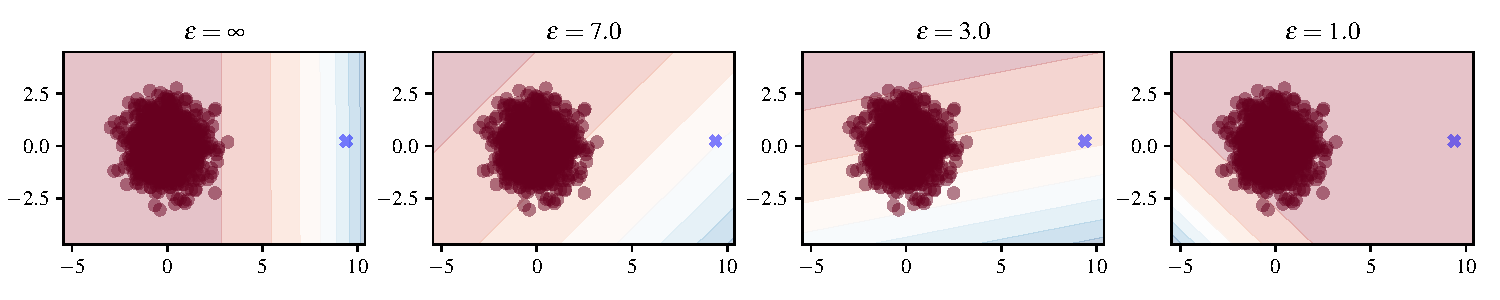
\includegraphics[width=\linewidth]{figs/sptd_dp/eps_gauss.pdf}
\caption[Synthetic example of privacy impacts on selective classification.]{\textbf{Synthetic example of privacy impacts on selective classification}. Shaded regions show softmax response confidence in the red and blue class, respectively. As $\varepsilon$ decreases, the blue outlier point is increasingly protected by DP. Importantly, not only does DP induce a misclassification on the outlier point, but stronger levels of DP further increase confidence in the wrong prediction. This overconfidence in the incorrect class prevents selective classification.}
\label{fig:eps_gauss}
\end{figure*}

%To summarize, in this experiment we saw a correlation between how the label ambiguity property affects the decision boundary, and how the performance of a specific SC method changes as a result.
% This is despite the models having the same utility level. 

%This example show that, even at an aligned utility level, stronger levels of differential privacy increasingly harm selective classification

%we see that, as we decrease $\varepsilon$, the influence of the outlier on the decision boundary also decreases. Note that all models $\varepsilon \in \{7,3,1\}$ misclassify the outlier, but, as $\varepsilon$ decreases, the model's confidence in the incorrect (red) class increases increases. This example shows that, even at an aligned utility level, stronger levels of differential privacy increasingly harm selective classification.
%: what is the impact of differential privacy on selective classification?

\subsection{How Should We Evaluate Selective Classification Under Differential Privacy?}
\label{sec:new_metric}

\begin{contriback}
This subsection was written with Anvith Thudi.
\end{contriback}



% \anvith{@stephan I think the transition/intro of this section is off? It's focusing on accuracy aligning being the key issue, where as the takeaway of the previous section is the possibility of accuracy not being the only effect of DP against SC. I would say that first, then have the question of "how do we disentangle the effect from accuracy to the overall effect on SC". You then can mention one way is to only ever consider models with the same accuracy, but it is known stronger privacy gives worse models and having to lower the accuracy of less private models may have unintended consequences (as described later in the accuracy-alignment results, and can describe the example of early stopping). Hence we propose a metric that is independent of accuracy which measures how close a method is to optimal for that given accuracy.} 

%In the previous section, we saw how DP can affect selective classification performance beyond just the implication from a degradation in baseline accuracy. 

As we have now established, we expect differential privacy to harm selective classification performance. %as a consequence of (i) the utility degradation it causes; but also (ii) the label ambiguity property of DP. 
In light of this insight, we are now investigating whether the standard evaluation scheme for SC is directly applicable to the differentially private models. %we are faced with the challenge of how to disentangle both effects from each other to arrive at a detailed characterization of the SC performance.
%induced from degrading accuracy to the overall effect on SC performance?
%potentially
%in ways independent of the degrading baseline utility. 
% In trying to understand this second cause, the question we are faced with is how to disentangle the effect induced from degrading accuracy to the overall effect on SC performance?

%The standard approach of using the current metric for SC performance (Equation~\ref{eq:sc_perf}) free of its bias towards accuracy is to accuracy-align the different models SC is being applied to. However, accuracy aligning can have unintended consequences on SC performance. In the case of models trained with DP, this would mean lowering the performance of the less private models. One approach to do this is by early-stopping model training at a desired accuracy level. But note, early-stopping a DP training algorithm in fact gives a model with greater privacy. This is as privacy loss accumulates during training, and so by training for less you have expended less privacy (i.e., end with a more private model). Hence instead of comparing models with different privacy guarantees at the same baseline utility, we have now models with potentially very similar privacy guarantees. \anvith{the previous sentence kind of assume people understand privacy loss} In short, accuracy aligning models can have unintended consequences that effect our ability to understand DP's role in degrading SC performance.

The default approach of using the SC performance metric introduced in Equation~\ref{eq:sc_perf} free from its bias towards accuracy is to align different SC approaches/models at the same accuracy. However, accuracy-aligning can have unintended consequences on SC performance, especially under DP. If we are considering SC performance across models trained for multiple $\varepsilon$ levels, accuracy-alignment would require lowering the performance of the less private models. One seemingly suitable approach to do this is by early-stopping model training at a desired accuracy level. However, early-stopping a DP training algorithm in fact gives a model with greater privacy than the privacy level targeted by the optimization process. This is a direct consequence of privacy loss accumulation via privacy accounting during training, and so training for less leads to expending less privacy budget. Hence, instead of comparing models with different privacy guarantees at the same baseline utility, early-stopping yields models with potentially very similar privacy guarantees. 
%In short, accuracy aligning models can have unintended consequences that affect our ability to understand DP's role in degrading SC performance.




%utility and selective classification performance. 


%Reconsidering the metric in Equation~\ref{eq:sc_perf}, we realize that this metric is a valid characterization of selective classification performance in accuracy-aligned experiments only. In particular, if and only if two selective classifiers $(f_i,g_i)$ and $(f_j,g_j)$ have the same full-coverage accuracy, \ie $\text{acc}_{c=1}(f_i,g_i) = \text{acc}_{c=1}(f_j,g_j)$, then Equation~\ref{eq:sc_perf} fully characterizes selective classification performance. In practice, aligning the full-coverage accuracy across models can be achieved by early-stopping model training at a desired accuracy level. 


%This need to align the full coverage utility across models creates challenges when it comes to evaluating DP models with varying degrees of privacy protection (i.e., varying upper bounds $\varepsilon$ on the privacy leakage). In particular, accuracy alignment under DP would require a constant model utility level across multiple $\varepsilon$s. However, contemporary privacy accounting techniques designed for sequential model training only exhaust the full privacy budget at the end of training. That is, for any step during the training process $t \in [T]$, the budget spent at time $t$, $\varepsilon_t$, is smaller than the final epsilon $\varepsilon=\varepsilon_T$, formally $\varepsilon_t < \varepsilon_T\ \forall t$. 
%Therefore, early-stopping a DP model yields a model that has not spent its full privacy budget $\varepsilon$. \stephan{I feel like there is still a step missing here} Hence, it is not possible to accuracy align models across $\epsilon$ levels and require a new performance metric that can account for this alignment issue. \stephan{@Anvith: maybe you can help me make this more rigorous?}


%This implies that early-stopping a model with final privacy budget $\epsilon$ in order to accuracy-align its utility with a model that spent its total final targeted privacy budget $\epsilon_2$ (with $\epsilon_1 > \epsilon_2$) would lead to a comparison of . 

% Old version
% As previously established, the addition of differential privacy negatively impacts model utility: as $\varepsilon$ decreases from $\infty$ (not private) to $0$ (fully private), the increased levels of clipping and noise addition in DP-SGD degrade model performance towards random-guessing accuracy. This unavoidable drop in accuracy presents a severe challenge to \anvith{"using"} the previously presented evaluation setup \anvith{"to compare the performance of the methods at different $\varepsilon$ values"}, \anvith{"as it" if you use the previous suggestions} which requires accuracy alignment across all evaluated models (\ie across $\varepsilon$ values). 
% In particular, we state that accuracy alignment under DP would require all models to be aligned to an accuracy value attainable from the most DP-constrained model, \ie the model with the lowest $\varepsilon$.
% The difficulty stems from the fact that, especially at low single-digit $\varepsilon$ values, no amount of early stopping or model architecture restriction can equalize full-coverage accuracy: as $\varepsilon$ decreases from $\infty$ (not private) to $0$ (fully private), the increased levels of clipping and noise addition in DP-SGD degrade model performance towards random-guessing accuracy. For example, as we discuss in more detail later, training a $(1,10^{-5})$-DP model and a non private model on CIFAR-10 does not allow for any accuracy alignment between the two models; the full coverage accuracy of the private model after exhausting the full privacy budget undercuts the utility level of the non-private model after a single epoch \anvith{this does not answer why you cannot use less than a single epoch}. 
% Moreover, accuracy alignment. via early stopping comes with additional restrictions of the employable selective classification algorithms. For instance, Selective Classification Training Dynamics relies on the intermediate predictions of a full training run in order to arrive at its scoring function $g$. Similarly, Self-Adaptive Training is designed with an initial burn-in phase in mind. Early stopping both methods early in training would therefore lead to considerable drops in selective classification performance.%the performance gap between a private and a non-private model on the same task can no restrictions to the model architecture

To address this limitation, %of the current metric for SC, 
we propose to measure SC performance by how close the observed trade-off is to an upper bound on the achievable SC performance at a given baseline utility level (at $100\%$ coverage). To compute this metric, we first derive an upper bound on selective classification performance (as a function of coverage) for a given baseline accuracy. We obtain this characterization by identifying the optimal acceptance ordering under a particular full-coverage accuracy constraint. %Deriving this ordering then gives an upper bound on the attainable selective classification performance. %At its core, the bound characterizes an optimal acceptance ordering under a particular full-coverage accuracy constraint. 
% \djcomment{Why is this called "optimal upper bound"? What is optimal about this? Can we formalize the notion of optimality being used here? If there isn't one, can we just call this a performance bound?}

\begin{figure}
\centering
% \begin{subfigure}%{0.48\textwidth}
\begin{minipage}{0.48\linewidth}      
{\centering
\small
\resizebox{\linewidth}{!}{
    \begin{tikzpicture}[
		declare function={}
		]
\begin{axis}[%
  xlabel=Coverage ($c$),
  ylabel=Accuracy,
  xmin = -0.1,
  xmax = 1.1,
  ymin = -0.1,
  ymax = 1.25,
  grid=major,
  width=8cm,
  height=5cm,
  tick label style={/pgf/number format/fixed},
  legend pos=north east]
  
  \newcommand\afull{0.4}
  \newcommand\afullinccoord{{\afull + (1 - \afull)/2}}
  
  \addplot+[mark={},dashed,line width=2pt,Black,name path=A, domain=0:\afull] {1};
  \addplot+[mark={},dashed,line width=2pt,Black,name path=B, domain=\afull:1] {\afull/x};
  \addplot+[draw=none,mark=none,name path=C,domain=0:1] {0};
  \addplot+[Green!25!white] fill between[of=A and C,soft clip={domain=0:\afull}];
  \addplot+[Red!25!white] fill between[of=B and C,soft clip={domain=\afull:1}];
  %\draw [black, line width=1pt, dashed] (\afull,0) -- (\afull, 1.0);
  \node[black, fill=white] at (1,\afull+0.13) {\scriptsize $a_\text{full}$};
  \node[black, fill=white] at (\afull,1.13) {\scriptsize $c = a_\text{full}$};

  % \addplot+[black,fill=black] coordinates{(\afull,1)};
  % \addplot+[black,fill=black] coordinates{(1,\afull)};

  \fill[black] (\afull, 1) circle[radius=2.5pt];
  \fill[black] (1,\afull) circle[radius=2.5pt];
  
  \draw [->, Red, line width=1pt] (\afull,0.05) -- (1, 0.05);
  \draw [->, Green, line width=1pt] (0,0.05) -- (\afull, 0.05);
  \node[Green] at (\afull/2,0.15) {\scriptsize correct points};
  \node[Red] at (\afullinccoord,0.15) {\scriptsize incorrect points};

  \legend{ \scriptsize \upperbound};
 
\end{axis}
\end{tikzpicture}
}}
    (a) \emph{Upper bound $\overline{\text{acc}}(a_\text{full},c)$ on the selective classification performance conditional on $a_\text{full}$}. As coverage $c$ increases from $0 \rightarrow 1$, an optimal selective classifier accepts all correct points first (with a consistent accuracy of $1$ until $c = a_\text{full}$) and then spreads the accuracy decrease $\frac{a_\text{full}}{c}$ equally over the remaining coverage spectrum, leading to a convex drop as $c \rightarrow 1$.
    \label{fig:bound}
\end{minipage}
% \end{subfigure}%
\hspace{10pt}
% \begin{subfigure}%{0.48\textwidth}
\begin{minipage}{0.48\linewidth}    
{\centering
\small
\resizebox{\linewidth}{!}{
\begin{tikzpicture}[
		declare function={}
		]
		\begin{axis}[%
		  xlabel=Coverage ($c$),
		  ylabel=Accuracy,
		  xmin = -0.1,
		  xmax = 1.1,
		  ymin = 0.3,
		  ymax = 1.1,
		  grid=major,
		  width=8cm,
		  height=5cm,
		  tick label style={/pgf/number format/fixed},
		  legend pos=north east]
		  
		  \newcommand\afull{0.4}
		  
		  \addplot+[mark={},line width=2pt,Black,name path=A, dashed, domain=0:\afull] {1};
		  %\addlegendentry{\scriptsize $\overline{\text{acc}}(a_\text{full},c)$}
		  \addplot+[mark={},line width=2pt,Black,name path=C, domain=0:\afull/2] {1};
		%\addlegendentry{\scriptsize $\text{acc}_c(f,g)$}
		  \addplot+[mark={},line width=2pt,Black,name path=B, dashed, domain=\afull:1] {\afull/x};
		  
		  
		  \addplot+[mark={},line width=2pt,Black,name path=D, domain=0.2:0.4] {15/16*x^2 - 15/8 * x + 107/80};
		  
		  \addplot+[mark={},line width=2pt,Black,name path=E, domain=0.4:1] {15/16*x^2 - 15/8 * x + 107/80};
		  
%		  \addplot+[Cyan!25!white] fill between[of=A and C,soft clip={domain=0:1}];
%		  \addplot+[Cyan!25!white] fill between[of=B and C,soft clip={domain=0:1}];
		  
		  \addplot+[Black!25!white] fill between[of=A and D,soft clip={domain=0:1}];
    % \legend{\scriptsize $\overline{\text{acc}}(a_\text{full},c)$, \scriptsize $\text{acc}_c(f,g)$, \scriptsize $s_{a_\text{full}}(f,g)$}
        \legend{ \scriptsize \upperbound, \scriptsize \empiricalacccovtradeoff, , , , \scriptsize \accnormscore };
		  \addplot+[Black!25!white] fill between[of=B and E,soft clip={domain=0:1}];
%		  \addplot+[Cyan!25!white] fill between[of=B and D,soft clip={domain=0:1}];
%		  \addplot+[Red!25!white] fill between[of=B and C,soft clip={domain=\afull:1}];
		 
		\end{axis}
		\end{tikzpicture}
    }}
    (b) \emph{Accuracy-normalizes score for SC performance.} The accuracy-normalized score for selective classification $s_{a_\text{full}}(f,g)$ corresponds to the area enclosed between the upper bound $\overline{\text{acc}}(a_\text{full},c)$ and the empirical accuracy/coverage trade-off $\text{acc}_c(f,g)$. Good selective classifiers should achieve a low score ($s_{a_\text{full}}(f,g) \approx 0$), indicating closeness to the bound.
    \label{fig:score}
\end{minipage}
\vspace{10pt}
% \end{subfigure}
    \caption[Selective classification upper bound and accuracy-normalized score visualization.]{\textbf{Selective classification upper bound and accuracy-normalized score visualization}. We present an example of a selective classifier with full-coverage accuracy $a_\text{full} = 0.4$ and show how (a)~the corresponding upper bound; and how (b) the accuracy-normalized score can be obtained. }
    \label{fig:bound_score}
\end{figure}

\begin{definition}
\emph{The upper bound on the selective classification performance for a fixed full-coverage accuracy $a_\text{full} \in [0,1]$ and a variable coverage level $c \in [0,1]$ is given by
    \begin{equation}
        \label{eq:sc_dp_bound}
        \overline{\text{acc}}(a_\text{full},c) = \begin{cases}
  1  & 0 < c \leq a_\text{full} \\
  \frac{a_\text{full}}{c} & a_\text{full} < c < 1
\end{cases}.
    \end{equation}
    }
\end{definition}
Measuring the area enclosed between the bound $\overline{\text{acc}}(a_\text{full},c)$ and an SC method's achieved accuracy/coverage trade-off $\text{acc}_c(f,g)$ yields our accuracy-normalized selective classification score. 
\begin{definition}
  \emph{The accuracy-normalized selective classification score $s_{a_\text{full}}(f,g)$ for a selective classifier $(f,g)$ with full-coverage accuracy $a_\text{full}$ is given by
  \begin{equation}
  \label{eq:acc_norm_score}
        s_{a_\text{full}}(f,g) = \int_0^1 (\overline{\text{acc}}(a_\text{full},c) - \text{acc}_c(f,g)) dc \approx \sum_c (\overline{\text{acc}}(a_\text{full},c) - \text{acc}_c(f,g)).
    \end{equation}
    }
\end{definition}
We provide additional intuition for both the proposed upper bound and our score as part of Figure~\ref{fig:bound_score}.

\paragraph{Bound justification.} To understand the upper bound given in Equation~\ref{eq:bound}, 
%assume the existence of a trained classification model with 
note that a full-coverage accuracy level of $a_\text{full}$ means that a fraction $a_\text{full}$ of points are correctly classified. %and $1-a_\text{full}$ of points are incorrectly classified. 
An ideal selective classification method for this model would, by increasing the coverage $c$ from 0 to 1, first accept all points that the model classifies correctly: this gives the optimal selective classification accuracy for coverage $c \leq a_{\text{full}}$ of $100\%$. 
%Hence, the accuracy of an optimal selective classifier is $1$ up to a coverage level of $a_\text{full}$. 
For any coverage level $c > a_{\text{full}}$, note that the accuracy at the coverage is the number of correct points accepted divided by the total number of points accepted. The largest value this can take is by maximizing the numerator, and the maximum value for this (as a fraction of all points) is $a_{\text{full}}$. Plugging this into the previous statement for accuracy at coverage $c$, we have the best selective accuracy at a coverage $c$ is $\frac{a_{\text{full}}}{c}$. This derives the upper bound stated above as a function of coverage. We remark that this bound is in fact achievable if a selective classifier separates correct and incorrect points perfectly, \ie it accepts all correct points first and then accepts and increasing amount of incorrect points as we increase the coverage of the selective classification method. See Appendix~\ref{sec:opt_bound_reach} for an experiment that matches the bound exactly. 
%We note that this metric is generally applicable beyond the study of DP models to any setting where evaluation across different accuracy levels is required. 

%After reaching a coverage level of $a_\text{full}$, the model has no choice but to accept all the points that the model predicted incorrectly on, i.e. the remaining $1-a_\text{full}$ fraction of points. Therefore, as we increase the coverage level from $a_\text{full}$ to 1, the optimal achievable accuracy is going to drop monotonically to the full-coverage accuracy level. In particular, the full-coverage accuracy $a_\text{full}$ needs to be distributed over the remaining coverage. This decay is therefore given by $\frac{a_\text{full}}{c}$.

% Coming back to our proposed approach of quantifying SC performance by measuring a SC method's closeness to the bound described above, we can measure the area enclosed between the bound $\overline{\text{acc}}(a_\text{full},c)$ and the method's achieved accuracy/coverage trade-off $\text{acc}_c(f,g)$. 
% \begin{definition}
%   \emph{The accuracy-normalized selective classification score $s_{a_\text{full}}(f,g)$ for a selective classifier $(f,g)$ with full-coverage accuracy $a_\text{full}$ is given by
%   \begin{equation}
%         s_{a_\text{full}}(f,g) = \int_0^1 (\overline{\text{acc}}(a_\text{full},c) - \text{acc}_c(f,g)) dc \approx \sum_c (\overline{\text{acc}}(a_\text{full},c) - \text{acc}_c(f,g)).
%     \end{equation}
%     }
% \end{definition}

%To quantify how optimal a SC method is, we can then compute the selective classification score for a selective classifier $(f,g)$ with full-coverage accuracy $a_\text{full}$ as the alignment between the bound $\overline{\text{acc}}(a_\text{full},c)$ and the selective accuracy of a particular model $\text{acc}_c(f,g)$, formally:
    
% Evaluating $s_{a_\text{full}}(f,g)$ for models reaching different levels of $a_\text{full}$ allows us to understand the effect that accuracy degradation has on selective classification. Hence, while this metric is generally applicable for settings where evaluation across different accuracy levels is required, this optimal distance score is of particular interest in a DP setting.
% \begin{figure*}[t]
%   \centering
%   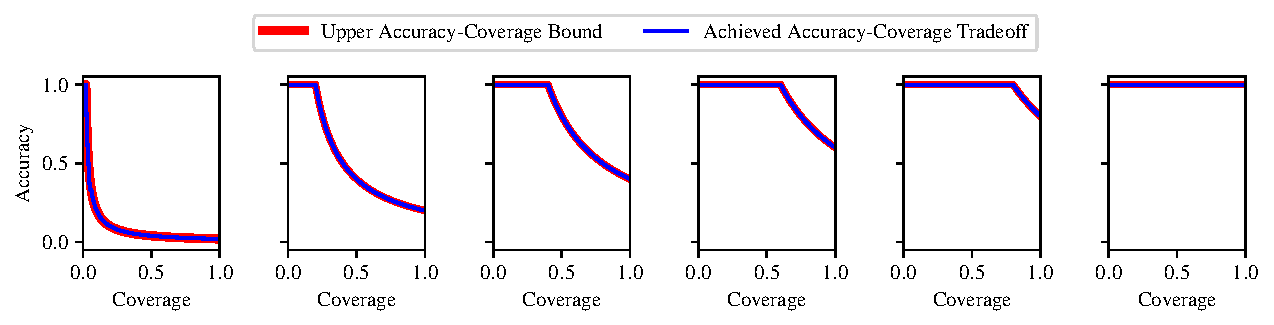
\includegraphics[width=\linewidth]{figs/sptd_dp/bound_reachability.pdf}
% \caption{\textbf{Text}. Text.}
% \label{fig:bound reachability}
% \end{figure*}

%This score now allows us to compare selective classification performance on models with varying full-coverage accuracy. That is, conditioned on the baseline utility of the model, how good is the model at identifying the optimal acceptance ordering for a given test set. %That is, this metric captures "how close is the method to optimal (for the given baseline utility of the model)".
%when considering the effectiveness of selective classification methods on models trained with varying DP guarantees, this metric allows us to answer how  optimal the methods become as the privacy guarantee changes. 

% \stephan{Look at last link in chain together}

% \stephan{Chain of thought starting below}

% \stephan{
% How is SC evaluated without DP? --> Accuracy-coverage trade-off, AUC under accuracy-coverage trade-off --> if we have different SC methods then we need to accuracy align to isolate the effect of SC}

% \stephan{
% We now understand how SC is evaluated --> now the goal is no longer to compare various SC methods against each other on the same task. instead we want to understand the how the SC capability of a model differs for a private and a non-private model --> the previous non-private method of evaluating SC performance relied on accuracy alignment --> is this possible under DP? --> yes, sometimes, if we compromise model utility of the non-private model --> we can compare across multiple privacy levels by aligning models with varying privacy guarantees to the model with the most conservative guarantee --> for the experiments where we can actually do this, we see that varying DP levels lead to the same SC performance trade-offs
% }

% \stephan{
% But this accuracy alignment is hard --> alignment requires under-fitting or model capacity restrictions on better performing models --> some SC methods do not work anymore because they rely on a full training run --> can we evaluate performance across various privacy guarantees leading to various accuracy levels? --> yes, we propose a new metric that does this --> this metric defines the optimal attainable selective classification behavior for a model under a particular full-coverage accuracy --> give method details --> while this is applicable even in non-private settings, DP leads to a wide spread in accuracies for varying epsilons --> this property makes this metric especially appealing in a DP setting
% }

% \stephan{
% If we compute this property, we see that as we decrease epsilon, all SC approaches perform progressively worse (larger distance to optimal bound) --> but there are other ways model accuracy can degrade (recall the alignment techniques we used which lead to lower accuracy) --> we see that they also move away from the bound --> therefore, our SC performance degradation observation is more general: accuracy degradation in current model (independent of the reason) degrades SC performance, too, as signified by a lager distance to the bound --> is the bound vacuous? is there even an optimal SC score that achieves this bound? --> yes, give synthetic example showing that we can get perfect SC performance even at low accuracy --> confirms that SC performance is far from solved in low-accuracy models --> can we say that less accurate models are more private? intuitively, this should be true. Early stopping: If we only train for 1-2 epochs then we have not spent the compute to enable memorization, which happens later in training. Simpler architectures: they don't have the ability to memorize the ability to memorize examples even after lengthy training (smaller train/test gap) --> more research needed
% }

\begin{figure*}[t]
  \centering
  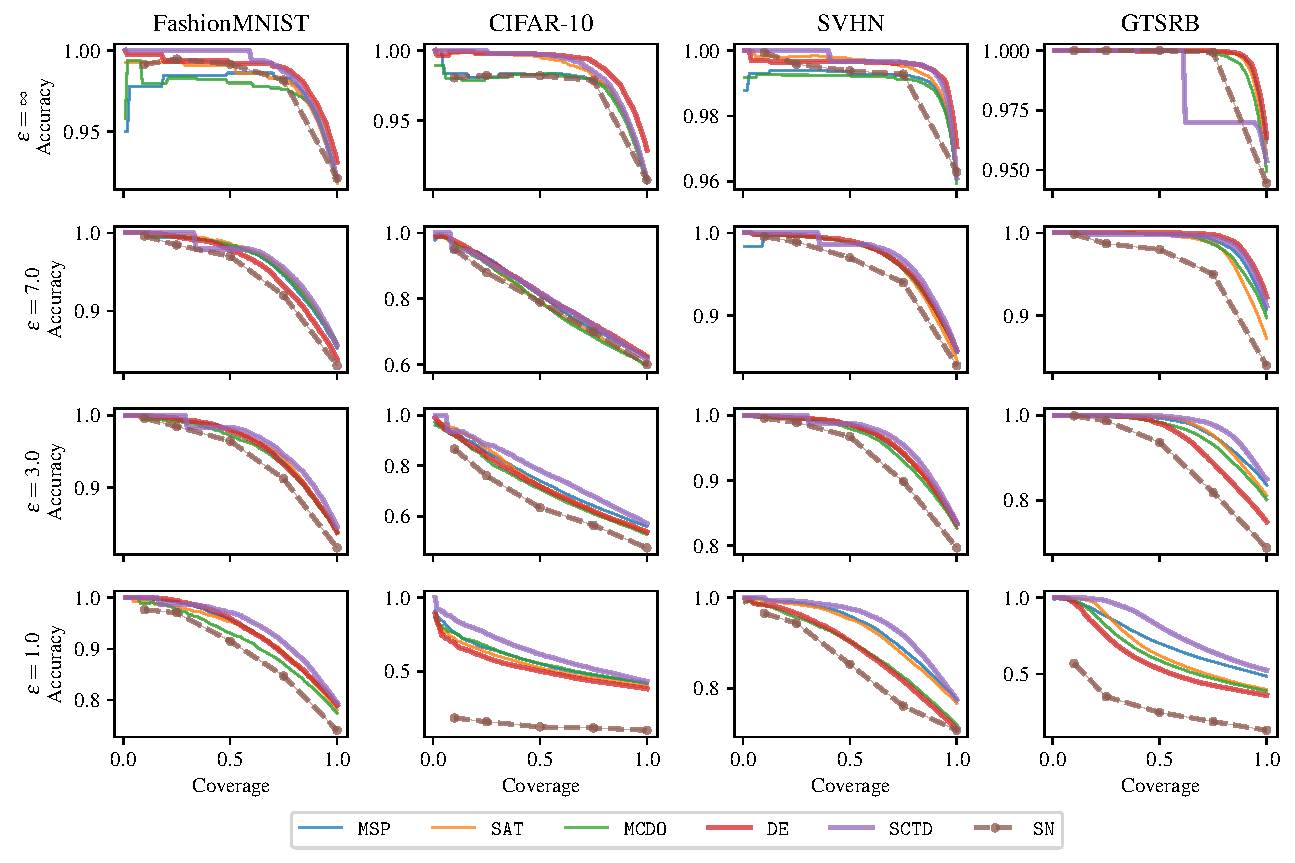
\includegraphics[width=\linewidth]{figs/sptd_dp/cov_acc.pdf}
\caption[Accuracy-coverage trade-off across datasets \& $\varepsilon$ levels.]{\textbf{Accuracy-coverage trade-off across datasets \& $\varepsilon$ levels}. We highlight noteworthy results for \sctd, \de, and \sn with bold lines and further show that \sn only provides results at coarse-grained coverage levels. \sctd performs best while \de and \sn performance is compromised at any $\varepsilon < \infty$.}
\label{fig:accuracy_coverage_tradeoff}
\end{figure*}

\section{Experiments}
\label{sec:exp}

We now present a detailed experimental evaluation of the interplay between differential privacy and selective classification. All of our experiments are implemented using PyTorch~\citep{Paszke_PyTorch_An_Imperative_2019} and Opacus~\citep{opacus}. We publish our full code-base at the following URL: \url{https://github.com/cleverhans-lab/selective-classification}.


\paragraph{Setup.} %We first present a detailed empirical evaluation of how current state-of-the-art selective classification techniques behave under various $\epsilon$-levels across multiple datasets. 
Our evaluation is based on the following experimental panel. In particular, we conduct experiments for each dataset/SC-method/$\varepsilon$ combination:
\begin{itemize}
    \item \textbf{Datasets}: FashionMNIST~\citep{xiao2017fashion}, CIFAR-10~\citep{krizhevsky2009learning}, SVHN~\citep{netzer2011reading}, GTSRB~\citep{Houben-IJCNN-2013}.
    \item \textbf{Selective Classification Methods}: Softmax Response (\sr)~\citep{geifman2017selective}, SelectiveNet (\sn)~\citep{geifman2019selectivenet}, Self-Adaptive Training (\sat)~\citep{huang2020self}, Monte-Carlo Dropout (\mcdo)~\citep{gal2016dropout}, Deep Ensembles (\de)~\citep{lakshminarayanan2017simple}, Selective Classification Training Dynamics (\sctd)~\citep{rabanser2022selective}.
    \item \textbf{Privacy levels}: $\varepsilon \in \{\infty, 7, 3, 1\}$.
\end{itemize}
% based on standard image datasets that are common in both the selective classification and differential privacy literature: FashionMNIST~\citep{xiao2017fashion}, CIFAR-10~\citep{krizhevsky2009learning}, SVHN~\citep{netzer2011reading}, and GTSRB~\citep{Houben-IJCNN-2013}. 
% \djcomment{Can we mention the methods as a list, its hard to read as is.}
% \djcomment{An outline at how this might look, ideally:
% \paragraph{Methods compared:}
% \begin{itemize}
%     \item SCTD ....
% \end{itemize}
% \paragraph{Privacy parameters used}
% \begin{itemize}
%     \item $\epsilon = \ldots, \delta=\ldots$
% \end{itemize}
% \paragraph{Architecture used}
% Resnet details
% \paragraph{Training parameters used}
% }
Based on recent results from~\citet{feng2023towards}, we (i) apply additional entropy regularization to all methods; and (ii) derive the selective classification scores for \sn and \sat by applying Softmax Response (\sr) to the underlying classifier (instead of relying on model-specific abstention mechanisms). Across all private experiments, we set $\delta = 10^{-(N+1)}$ for datasets consisting of training samples on the order of $10^N$. For each combination of SC method, dataset, and privacy level, we train a model following the ResNet-18~\citep{he2016deep} model architecture using either the SGD optimizer (for $\varepsilon=\infty$) or the DP-SGD optimizer (for all $\varepsilon<\infty$). All models are trained for 200 epochs using a mini-batch size of 128. For all DP training runs, we set the clipping norm to $c=10$ and choose the noise multiplier adaptively to reach the overall privacy budget at the end of training. Note that, since we want to consider a consistent value of $\varepsilon$ across all SC methods, we restrict the overall $\varepsilon$ in both \sn and \de. As explained in Section~\ref{sec:sc_affects_dp}, this effectively enforces a reduction in $\varepsilon$ for each individual training run due to sequential composition. Concretely, we train \de with 5 ensemble members and \sn with target coverage levels $c_\text{target} \in \{0.1,0.25,0.5,0.75,1.0\}$. This leads to a reduction of $\approx\frac{\varepsilon}{\sqrt 5}$ for each trained sub-model in both cases. We account for the precise reduction in the privacy parameter by~\emph{increasing by the number steps of DP-SGD} as measured by a R\'enyi DP accountant~\citep{mironov2017renyi,opacus}. % by factor of $5$. 
All experiments are repeated over 5 random seeds to determine the statistical significance of our findings. We document additional %SC-method-specific and other 
hyper-parameters in Appendix~\ref{sec:hyp}.

% \begin{table}[t]
%     % \tiny
%     \fontsize{5.5}{6}\selectfont
% \tabcolsep=0.08cm
%         \caption{\textbf{Coverage required for non-private full-coverage accuracy.} We observe that differential privacy considerably lowers the allowable coverage to achieve a utility level consistent with the non-private model. Across our experiments, \sctd yields the highest coverage across $\varepsilon$ levels.}
%         \vspace{5pt}
%         \centering
%         \label{tab:coverage_performance}
% \begin{tabular}{ccccccccccccc}
% \toprule
%  & \multicolumn{3}{c}{FashionMNIST} & \multicolumn{3}{c}{CIFAR-10} & \multicolumn{3}{c}{SVHN} & \multicolumn{3}{c}{GTSRB} \\ 
% \cmidrule(lr){2-4} \cmidrule(lr){5-7} \cmidrule(lr){8-10} \cmidrule(lr){11-13}
%  & $\varepsilon = 7$ & $\varepsilon = 3$ & $\varepsilon = 1$ & $\varepsilon = 7$ & $\varepsilon = 3$ & $\varepsilon = 1$ & $\varepsilon = 7$ & $\varepsilon = 3$ & $\varepsilon = 1$ & $\varepsilon = 7$ & $\varepsilon = 3$ & $\varepsilon = 1$ \\
% \midrule
% \msp & 0.83 (±0.01) & 0.80 (±0.01) & 0.65 (±0.03) & \bfseries 0.29 (±0.02) & 0.14 (±0.04) & 0.00 (±0.00) & 0.74 (±0.00) & 0.67 (±0.01) & 0.49 (±0.02) & 0.90 (±0.01) & 0.71 (±0.03) & 0.13 (±0.00) \\
% \sat & \bfseries 0.86 (±0.00) & 0.81 (±0.01) & 0.67 (±0.02) & 0.25 (±0.01) & \bfseries 0.19 (±0.02) & 0.00 (±0.00) & 0.72 (±0.00) & 0.67 (±0.01) & 0.45 (±0.02) & 0.86 (±0.00) & 0.74 (±0.00) & 0.20 (±0.03) \\
% \mcdo & \bfseries 0.84 (±0.02) & 0.79 (±0.00) & 0.56 (±0.02) & 0.25 (±0.01) & 0.12 (±0.02) & 0.00 (±0.00) & 0.74 (±0.00) & 0.64 (±0.00) & 0.23 (±0.03) & 0.90 (±0.01) & 0.69 (±0.01) & 0.14 (±0.01) \\
% \de & 0.75 (±0.00) & 0.75 (±0.01) & 0.61 (±0.01) & 0.22 (±0.01) & 0.09 (±0.00) & 0.00 (±0.00) & 0.69 (±0.01) & 0.62 (±0.01) & 0.22 (±0.00) & \bfseries 0.93 (±0.00) & 0.57 (±0.08) & 0.10 (±0.04) \\
% \sctd & \bfseries 0.86 (±0.01) & \bfseries 0.84 (±0.02) & \bfseries 0.73 (±0.01) & \bfseries 0.26 (±0.03) & \bfseries 0.20 (±0.03) & \bfseries 0.04 (±0.04) & \bfseries 0.78 (±0.01) & \bfseries 0.72 (±0.00) & \bfseries 0.59 (±0.02) & \bfseries 0.93 (±0.01) & \bfseries 0.83 (±0.03) & \bfseries 0.30 (±0.02) \\
% \bottomrule
% \end{tabular}
% \end{table}

\begin{table}[t]
    \fontsize{8.5}{8}\selectfont
    \tabcolsep=0.175cm
    \caption[Coverage required for non-private full-coverage accuracy.]{\textbf{Coverage required for non-private full-coverage accuracy.} We observe that differential privacy considerably lowers the allowable coverage to achieve a utility level consistent with the non-private model. Across our experiments, \sctd yields the highest coverage across $\varepsilon$ levels.}
    \vspace{5pt}
    \centering
    \label{tab:coverage_performance}
    \begin{tabular}{c c c c c c c}
    \toprule
    % \multicolumn{7}{c}{\textbf{FashionMNIST \& CIFAR-10}} \\
    % \cmidrule(lr){1-7}
    & \multicolumn{3}{c}{FashionMNIST} & \multicolumn{3}{c}{CIFAR-10} \\
    \cmidrule(lr){2-4} \cmidrule(lr){5-7}
           & $\varepsilon=7$ & $\varepsilon=3$ & $\varepsilon=1$ & $\varepsilon=7$ & $\varepsilon=3$ & $\varepsilon=1$ \\
    \midrule
    \msp  & 0.83 (±0.01) & 0.80 (±0.01) & 0.65 (±0.03) & \bfseries 0.29 (±0.02) & 0.14 (±0.04) & 0.00 (±0.00) \\
    \sat  & \bfseries 0.86 (±0.00) & 0.81 (±0.01) & 0.67 (±0.02) & 0.25 (±0.01) & \bfseries 0.19 (±0.02) & 0.00 (±0.00) \\
    \mcdo & \bfseries 0.84 (±0.02) & 0.79 (±0.00) & 0.56 (±0.02) & 0.25 (±0.01) & 0.12 (±0.02) & 0.00 (±0.00) \\
    \de   & 0.75 (±0.00) & 0.75 (±0.01) & 0.61 (±0.01) & 0.22 (±0.01) & 0.09 (±0.00) & 0.00 (±0.00) \\
    \sctd & \bfseries 0.86 (±0.01) & \bfseries 0.84 (±0.02) & \bfseries 0.73 (±0.01) & \bfseries 0.26 (±0.03) & \bfseries 0.20 (±0.03) & \bfseries 0.04 (±0.04) \\
    % \midrule
    % \multicolumn{7}{c}{\textbf{SVHN \& GTSRB}} \\
    % \cmidrule(lr){1-7}
    \cmidrule(lr){2-4} \cmidrule(lr){5-7}
    & \multicolumn{3}{c}{SVHN} & \multicolumn{3}{c}{GTSRB} \\
    \cmidrule(lr){2-4} \cmidrule(lr){5-7}
    %        & $\varepsilon=7$ & $\varepsilon=3$ & $\varepsilon=1$ & $\varepsilon=7$ & $\varepsilon=3$ & $\varepsilon=1$ \\
    % \midrule
    \msp  & 0.74 (±0.00) & 0.67 (±0.01) & 0.49 (±0.02) & 0.90 (±0.01) & 0.71 (±0.03) & 0.13 (±0.00) \\
    \sat  & 0.72 (±0.00) & 0.67 (±0.01) & 0.45 (±0.02) & 0.86 (±0.00) & 0.74 (±0.00) & 0.20 (±0.03) \\
    \mcdo & 0.74 (±0.00) & 0.64 (±0.00) & 0.23 (±0.03) & 0.90 (±0.01) & 0.69 (±0.01) & 0.14 (±0.01) \\
    \de   & 0.69 (±0.01) & 0.62 (±0.01) & 0.22 (±0.00) & \bfseries 0.93 (±0.00) & 0.57 (±0.08) & 0.10 (±0.04) \\
    \sctd & \bfseries 0.78 (±0.01) & \bfseries 0.72 (±0.00) & \bfseries 0.59 (±0.02) & \bfseries 0.93 (±0.01) & \bfseries 0.83 (±0.03) & \bfseries 0.30 (±0.02) \\
    \bottomrule
    \end{tabular}
\end{table}


\paragraph{Evaluation of selective classification techniques across privacy levels.}

We report our main results in Figure~\ref{fig:accuracy_coverage_tradeoff} where we display the accuracy-coverage trade-off for our full experimental panel. Overall, we observe that Selective Classification Training Dynamics (\sctd) delivers the best accuracy-coverage trade-offs. While this is consistent with non-private~\citep{rabanser2022selective}, we find that \sctd delivers especially strong performance at lower $\varepsilon$ levels. This suggests that leveraging training dynamics information is useful for performative selective classification under DP. As expected, based off of the discussion in Section~\ref{sec:sc_affects_dp}, Figure~\ref{fig:accuracy_coverage_tradeoff} also shows that the performance of both Deep Ensembles (\de) and SelectiveNet (\sn) suffers under DP, showing increasing utility degradation as $\varepsilon$ decreases. %In particular, for GTSRB trained using $(1,\delta)$-DP, both models never exceed random guessing accuracy.

% \begin{table}[t]
%     \scriptsize
% \fontsize{6.5}{6}\selectfont
%     \tabcolsep=0.1cm
% \caption{\textbf{Accuracy-normalized selective classification performance.} Across our panel of  experiments, we find that decreasing $\varepsilon$ leads to a worse (\ie higher) score, meaning that as $\varepsilon$ decreases the selective classification approaches all move away from the upper bound.}
% \vspace{5pt}
%         \centering
%         \label{tab:sc_score_performance}
%         \begin{tabular}{ccccccccc}
% \toprule
%  & \multicolumn{4}{c}{FashionMNIST} & \multicolumn{4}{c}{CIFAR-10} \\
% \cmidrule(lr){2-5} \cmidrule(lr){6-9}
%  & $\epsilon = \infty$ & $\epsilon = 7$ & $\epsilon = 3$ & $\epsilon = 1$ & $\epsilon = \infty$ & $\epsilon = 7$ & $\epsilon = 3$ & $\epsilon = 1$ \\
% \midrule
% \msp & 0.019 (±0.000) & 0.023 (±0.000) & 0.027 (±0.002) & 0.041 (±0.001) & 0.019 (±0.000) & 0.105 (±0.002) & 0.133 (±0.002) & 0.205 (±0.001) \\
% \sat & 0.014 (±0.000) & \bfseries 0.020 (±0.001) & 0.026 (±0.002) & 0.043 (±0.002) & 0.010 (±0.000) & 0.107 (±0.000) & 0.128 (±0.000) & 0.214 (±0.002) \\
% \mcdo & 0.020 (±0.002) & 0.023 (±0.001) & 0.030 (±0.003) & 0.053 (±0.001) & 0.021 (±0.001) & 0.110 (±0.000) & 0.142 (±0.000) & 0.201 (±0.000) \\
% \de & \bfseries 0.010 (±0.003) & 0.027 (±0.002) & 0.027 (±0.002) & 0.039 (±0.000) & \bfseries 0.007 (±0.001) & \bfseries 0.099 (±0.002) & 0.138 (±0.000) & 0.222 (±0.000) \\
% \nntd & \bfseries 0.007 (±0.001) & \bfseries 0.021 (±0.001) & \bfseries 0.023 (±0.003) & \bfseries 0.032 (±0.002) &  \bfseries 0.009 (±0.002) & \bfseries 0.098 (±0.001) & \bfseries 0.107 (±0.001) & \bfseries 0.152 (±0.001) \\
% \sn & \bfseries 0.008 (±0.002) & 0.058 (±0.001) & 0.056 (±0.001) & 0.064 (±0.002) & 0.015 (±0.000) & 0.155 (±0.003) & 0.154 (±0.002) & 0.173 (±0.001) \\

% \cmidrule(lr){2-5} \cmidrule(lr){6-9}
% & \multicolumn{4}{c}{SVHN} & \multicolumn{4}{c}{GTSRB} \\
% \cmidrule(lr){2-5} \cmidrule(lr){6-9}
% \msp & 0.008 (±0.001) & 0.020 (±0.001) & 0.024 (±0.001) & 0.040 (±0.001) & \bfseries  0.001 (±0.001) & 0.006 (±0.002) & 0.017 (±0.000) & 0.109 (±0.002) \\
% \sat & \bfseries 0.004 (±0.000) & 0.019 (±0.000) & \bfseries 0.021 (±0.002) & 0.044 (±0.002) & \bfseries  0.001 (±0.001) & 0.008 (±0.001) & 0.014 (±0.000) & 0.089 (±0.000) \\
% \mcdo & 0.009 (±0.000) & 0.019 (±0.001) & 0.027 (±0.002) & 0.069 (±0.001) & 0.002 (±0.001) & 0.007 (±0.001) & 0.023 (±0.001) & 0.110 (±0.001) \\
% \de & \bfseries 0.004 (±0.001) & 0.018 (±0.001) & \bfseries 0.022 (±0.002) & 0.067 (±0.003) & \bfseries 0.001 (±0.000) & \bfseries 0.003 (±0.002) & 0.027 (±0.004) & 0.127 (±0.002) \\
% \nntd & \bfseries 0.003 (±0.001) & \bfseries 0.016 (±0.001) & \bfseries 0.018 (±0.002) & \bfseries 0.027 (±0.001) & 0.011 (±0.002) & \bfseries 0.005 (±0.000) & \bfseries 0.009 (±0.000) & \bfseries 0.062 (±0.001) \\
% \sn & \bfseries 0.004 (±0.000) & 0.055 (±0.001) & 0.052 (±0.000) & 0.096 (±0.000) & \bfseries 0.001 (±0.001) & 0.050 (±0.004) & 0.044 (±0.001) & 0.091 (±0.004) \\
% \bottomrule
% \end{tabular}
% \end{table}

\begin{table}[t]
    \scriptsize
    \fontsize{7}{6.5}\selectfont
    \tabcolsep=0.145cm
\caption[Accuracy-normalized selective classification performance.]{\textbf{Accuracy-normalized selective classification performance.} Across our panel of experiments, we find that decreasing \(\varepsilon\) leads to a worse (\ie higher) score, meaning that as \(\varepsilon\) decreases the selective classification approaches all move away from the upper bound.}
\vspace{5pt}
    \centering
    \label{tab:sc_score_performance}
    \begin{tabular}{ccccccc}
\toprule
 & \multicolumn{3}{c}{FashionMNIST} & \multicolumn{3}{c}{CIFAR-10} \\
\cmidrule(lr){2-4} \cmidrule(lr){5-7}
 & \(\varepsilon = \infty\) & \(\varepsilon = 7\) & \(\varepsilon = 1\) & \(\varepsilon = \infty\) & \(\varepsilon = 7\) & \(\varepsilon = 1\) \\
\midrule
\msp  & 0.019 (±0.000) & 0.023 (±0.000) & 0.041 (±0.001) & 0.019 (±0.000) & 0.105 (±0.002) & 0.205 (±0.001) \\
\sat  & 0.014 (±0.000) & \bfseries 0.020 (±0.001) & 0.043 (±0.002) & 0.010 (±0.000) & 0.107 (±0.000) & 0.214 (±0.002) \\
\mcdo & 0.020 (±0.002) & 0.023 (±0.001) & 0.053 (±0.001) & 0.021 (±0.001) & 0.110 (±0.000) & 0.201 (±0.000) \\
\de   & \bfseries 0.010 (±0.003) & 0.027 (±0.002) & 0.039 (±0.000) & \bfseries 0.007 (±0.001) & \bfseries 0.099 (±0.002) & 0.222 (±0.000) \\
\nntd & \bfseries 0.007 (±0.001) & \bfseries 0.021 (±0.001) & \bfseries 0.032 (±0.002) & \bfseries 0.009 (±0.002) & \bfseries 0.098 (±0.001) & \bfseries 0.152 (±0.001) \\
\sn   & \bfseries 0.008 (±0.002) & 0.058 (±0.001) & 0.064 (±0.002) & 0.015 (±0.000) & 0.155 (±0.003) & 0.173 (±0.001) \\
    \cmidrule(lr){2-4} \cmidrule(lr){5-7}
    & \multicolumn{3}{c}{SVHN} & \multicolumn{3}{c}{GTSRB} \\
    \cmidrule(lr){2-4} \cmidrule(lr){5-7}
\msp  & 0.008 (±0.001) & 0.020 (±0.001) & 0.040 (±0.001) & \bfseries 0.001 (±0.001) & 0.006 (±0.002) & 0.109 (±0.002) \\
\sat  & \bfseries 0.004 (±0.000) & 0.019 (±0.000) & 0.044 (±0.002) & \bfseries 0.001 (±0.001) & 0.008 (±0.001) & 0.089 (±0.000) \\
\mcdo & 0.009 (±0.000) & 0.019 (±0.001) & 0.069 (±0.001) & 0.002 (±0.001) & 0.007 (±0.001) & 0.110 (±0.001) \\
\de   & \bfseries 0.004 (±0.001) & 0.018 (±0.001) & 0.067 (±0.003) & \bfseries 0.001 (±0.000) & \bfseries 0.003 (±0.002) & 0.127 (±0.002) \\
\nntd & \bfseries 0.003 (±0.001) & \bfseries 0.016 (±0.001) & \bfseries 0.027 (±0.001) & 0.011 (±0.002) & \bfseries 0.005 (±0.000) & \bfseries 0.062 (±0.001) \\
\sn   & \bfseries 0.004 (±0.000) & 0.055 (±0.001) & 0.096 (±0.000) & \bfseries 0.001 (±0.001) & 0.050 (±0.004) & 0.091 (±0.004) \\
\bottomrule
\end{tabular}
\end{table}



\begin{figure*}[t]
  \centering
  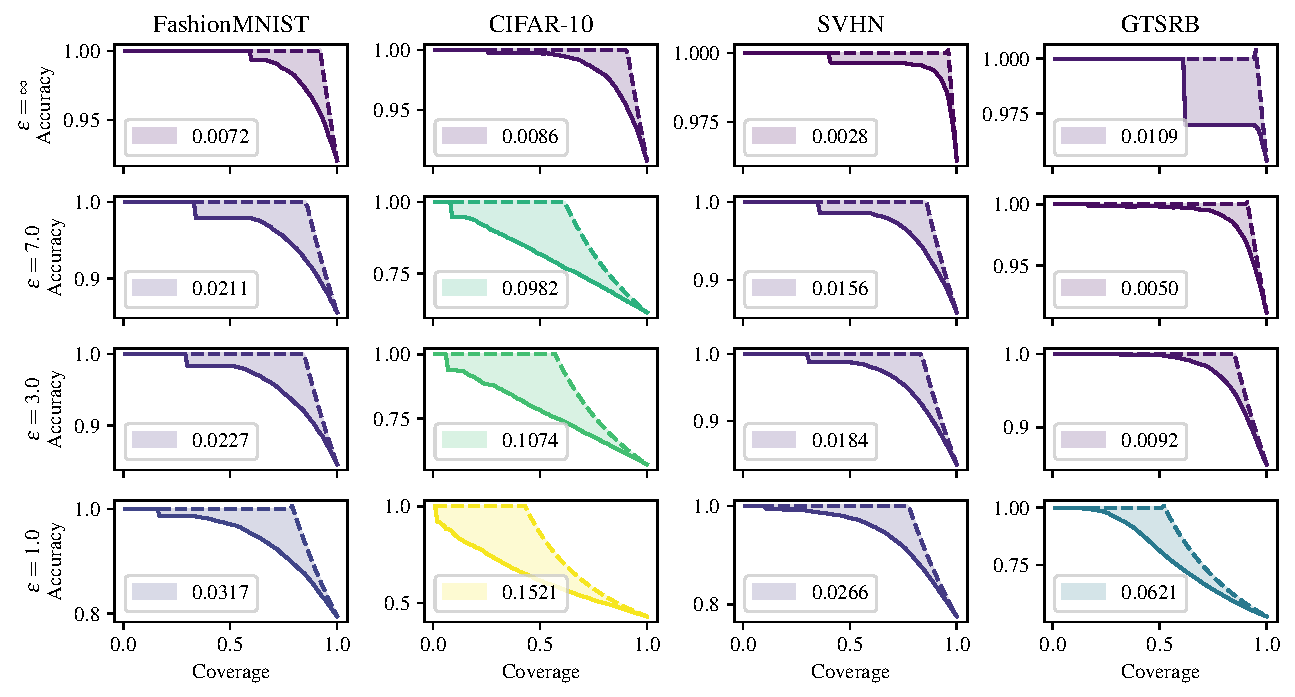
\includegraphics[width=\linewidth]{figs/sptd_dp/cov_acc_bound.pdf}
\caption[Distance to accuracy-dependent upper bound for the \sctd method.]{\textbf{Distance to accuracy-dependent upper bound for the \sctd method.} We plot both the accuracy-coverage trade-off of \sctd, \ie $\text{acc}_c(f,g)$, with a solid line and the upper bound $\overline{\text{acc}}(a_\text{full},c)$ with a dashed line. The shaded region enclosed between the two curves corresponds to the accuracy-normalized SC score $s_{a_\text{full}}(f,g)$. We observe that the score grows with stronger DP levels (shown by brighter colors), \ie selective classification becomes harder at low $\varepsilon$s.}
\label{fig:acc_cov_bound}
\end{figure*}

\paragraph{Recovering non-private utility by reducing coverage.}

Recall that one key motivation for applying selective classification to a DP model is to recover non-private model utility at the expense of coverage. We investigate this coverage cost in detail by examining how many samples a DP model can produce decisions for while maintaining the utility level of the respective non-private model (\ie a model trained on the same dataset without DP). The results are outlined in Table~\ref{tab:coverage_performance}. For high (\ie $\varepsilon=7$) and moderate (\ie $\varepsilon=3$) privacy budgets, we observe that a reduction of $20\%-30\%$ in data coverage recovers non-private utility. However, at low (\ie $\varepsilon=1$) privacy budget we observe that dataset coverage degrades strongly on most datasets. In particular, we find that for CIFAR-10 (across all $\varepsilon$ values) and GTSRB (at $\varepsilon=1$), the coverage reduces to below $30\%$. This result showcases that, depending on the particular choice of $\varepsilon$, recovering non-private model performance from a DP model can come at a considerable coverage cost. Moreover, this coverage cost varies widely across SC methods with \sctd leading to the lowest incurred loss in coverage by far.

\paragraph{Disentangling selective prediction performance from base accuracy.}

Recall from Section~\ref{sec:new_metric} that the standard evaluation pipeline for selective classification is not suitable for comparing DP models across varying privacy guarantees. To overcome this issue, we compute the accuracy-dependent upper bound (Equation~\ref{eq:sc_dp_bound}) for each experiment and measure how closely the achieved accuracy/coverage trade-off aligns with this bound as per Equation~\ref{eq:acc_norm_score}. We document these results computed over all datasets, SC methods, and $\varepsilon$ levels in Table~\ref{tab:sc_score_performance}. We find that, as $\varepsilon$ decreases, all methods perform progressively worse. That is, for stronger privacy, all methods increasingly struggle to identify points they predict correctly on. Recall that this behavior is expected based on our discussion in Section~\ref{sec:dp_affects_sc}. Again, we observe \sctd offering the strongest results, leading to the smallest bound deviation. To graphically showcase closeness to the upper bound, we further plot the accuracy-coverage trade-off and the corresponding upper bound for each experiment with the \sctd method in Figure~\ref{fig:acc_cov_bound}. 

\begin{figure*}[t]
  \centering
  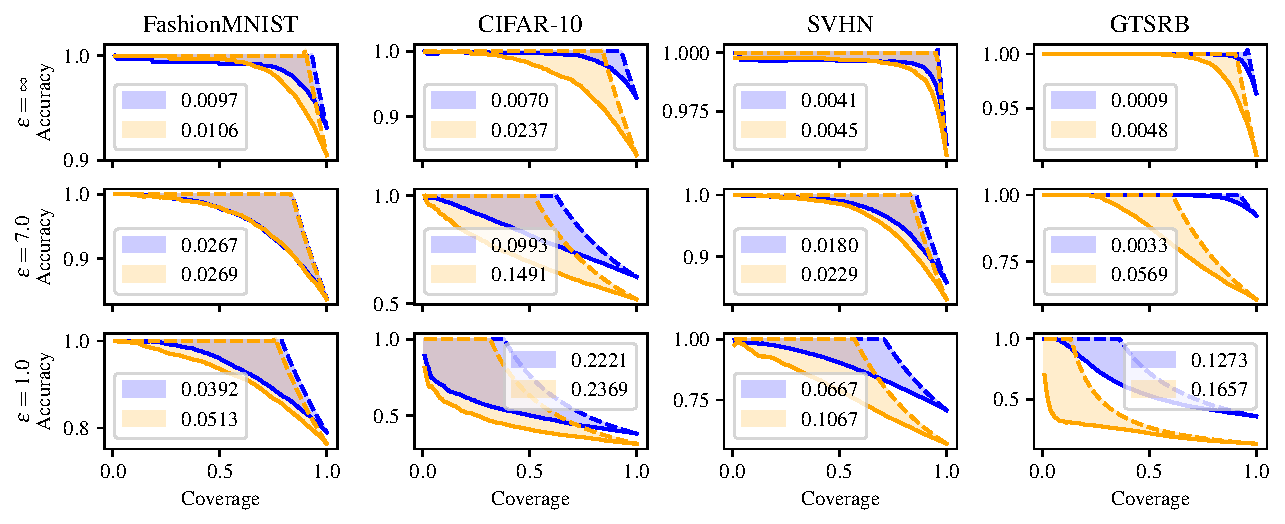
\includegraphics[width=\linewidth]{figs/sptd_dp/cov_acc_de_bound}
\caption[Sequential composition (\de) vs parallel composition (\texttt{DE-PART}) for deep ensembles.]{\textbf{Sequential composition (\de) vs parallel composition (\texttt{DE-PART}) for deep ensembles.} We observe that \texttt{DE-PART} (orange) under-performs \de (blue) for selective classification across all $\varepsilon$.}
\label{fig:acc_cov_bound_de}
\end{figure*}

\paragraph{Parallel composition with partitioned ensembles.}

As previously stated, Deep Ensembles under-perform under DP due to composition. One potential mitigation strategy is to partition the data and train isolated models with no data overlap. This circumvents composition but also limits the utility of individual ensemble members as less data is available for training. We experiment with both setups and report results in Figure~\ref{fig:acc_cov_bound_de}. Overall, these experimental results indicate that (i) partitioned deep ensembles lead to lower full-coverage accuracy when compared to non-partitioned deep ensembles while (ii) at the same time being less performant in terms of selective classification performance.

%, stronger degrees of privacy lead to worse SC performance as measured by the accuracy-dependent bound-closeness score. %Hence, we conclude that differentially private models do not know what they do not know.

% Based on the selective classification score reported in Table~\ref{tab:sc_score_performance}, we see that, across SC methods and datasets, the accuracy-normalized selective classification score increases as $\epsilon$ decreases. This confirms that differential privacy does not only lower full-coverage accuracy but further deteriorates our ability to perform selective classification.

% \subsection{Is the Optimal Bound Gap Necessarily Induced By Privacy?}

% The previous results raise an interesting question: is the larger discrepancy with respect to the optimal bound a direct cause of differentially private training? To shed some light on this question, we examine the optimal selective classification performance under a accuracy degradation that is not caused by DP. In particular, we investigate the effect of training a model with early stopping with accuracy alignment.  Future work should investigate whether models that are trained (i) using only a small number of overall mini-batches; or (ii) using a more simple model architecture offer comparable privacy guarantees.

% \stephan{Experiment 1: Big panel of SC methods for various datasets across different epsilon levels. Ideally shows us:
% \begin{itemize}
%     \item Main: Which SC methods perform well: should confirm that DeepEnsembles and SelectievNet degrades under stronger privacy. NNTD performs well.
%     \item Secondary, sanity check: Accuracy degrades with lower epsilon
% \end{itemize}
% }

% \stephan{Experiment 2: At what coverage cost can we recover the performance of a non-private model
% }

% \stephan{Experiment 3: We saw in exp 1 that accuracy degrades, as expected. Compute accuracy-normalized score which isolated the SC performance. Ideally shows us:
% \begin{itemize}
%     \item That distance to bound gets larger at lower privacy levels. DP makes selective classification harder
% \end{itemize}
% }

% \stephan{Experiment 4: Is the drop just because of DP? Or do we see that same drop for other methods that are accuracy aligned? I.e. do other methods that reduce accuracy also lead to sub-optimal performance at low accuracy levels. Seems to show us:
% \begin{itemize}
%     \item If accuracy alignment is possible, then the SC trends are the same. 
% \end{itemize}
% }

% \stephan{Experiment 5: Can we measure the privacy of all these accuracy-aligned methods? Simple membership inference based on the MSP?
% }

% \stephan{Experiment 6: Is the optimal bound attainable? Yes, we can present a simple experiment that does this at any desired accuracy level.
% }


\section{Conclusion}
\label{sec:concl}

In this work we have studied methods for performing selective classification under a differential privacy constraint. To that end, we have highlighted the fundamental difficulty of performing selective prediction under differential privacy, both via a synthetic example and empirical studies. To enable this analysis, we introduced a novel score that disentangles selective classification performance from baseline utility. While we establish that SC under DP is indeed challenging, our study finds that a specific method (\sctd) achieves the best trade-offs between SC performance and privacy budget. %owing largely to the fact that it only using information from a single training run and does not require training multiple models. 

\paragraph{Limitations.} This work presents insights drawn from empirical results and we acknowledge that a more thorough theoretical analysis is needed for a deeper understanding of the interplay between SC and DP. Also, we did not carefully investigate fairness implications beyond class imbalance. This connection to fairness requires special attention with past works showing that both DP and SC can negatively affect sensitive subgroups~\citep{jones2020selective, bagdasaryan2019differential}.

\paragraph{Future work.} We believe that this work initiates a fruitful line of research. 
%towards improving differentially private ML models, by endowing them with the ability to abstain instead of being forced to make an incorrect prediction when it is infeasible to do so under DP. 
In particular, future work can expand on the intuition provided here to obtain fundamental bounds on selective classification performance in a DP setting. Although we did not focus on this here, we believe that the ideas developed in this chapter could help mitigate the trade-offs between privacy and subgroup fairness.
%By abstaining from making confident predictions on underrepresented subgroups where differential privacy makes learning hard, we endow DP ML models to provide better transparency to individuals in underrepresented groups.

%We have studied methods for performing selective classification under a differential privacy constraint. We have also highlighted the fundamental difficulty of performing selective prediction under differential privacy, both via a theoretical example and empirical studies in Section 4.2. While the problem is indeed challenging, our study finds that a specific method (SCTD) achieves the best tradeoffs between selective prediction performance and privacy budget $(\epsilon, \delta)$, owing largely to the fact that it only using information from a single training run and does not require training multiple models or heads. We believe that this work initiates a fruitful line of research towards improving differentially private ML models, by endowing them with the ability to say "I don't know" instead of being forced to make an incorrect prediction when it is infeasible to do so under a privacy constraint. Further research can expand on the intuition provided here to obtain fundamental bounds on selective classification performance in a differential private setting. Although we did not focus on this here, we believe that the ideas developed in this paper are a promising route to mitigating the tradeoffs between privacy and subgroup fairness. By abstaining from making confident predictions on underrepresented subgroups where differential privacy makes learning hard, we endow DP ML models to provide better transperancy to individuals in underrepresented groups. 
% }